% Autor: Carles Marin (Claude, Anthropic, como asistente de investigacion IA).
% Version en castellano de "One Row of Their Table: proton stability in SU(7) grand gauge-Higgs
% unification". Traduccion COMPLETA, no resumen: arXiv exige el articulo entero en ambos idiomas.
% Las figuras son las variantes _es, generadas por ../make_figures_su7.py --es desde el mismo JSON
% archivado; ningun numero se recomputa ni se transcribe al traducir.
% Build: pdflatex x2.  Verificadores: check_numbers.py, check_refs.py, check_layout.py.
\documentclass[11pt,a4paper]{article}
\usepackage{cmap}   % ToUnicode CMaps: sin esto las ligaduras fi/fl/ffi de T1 no se extraen ni se buscan
\usepackage[utf8]{inputenc}
\usepackage[T1]{fontenc}
\usepackage[spanish,es-noquoting,es-nodecimaldot]{babel}
\usepackage{amsmath,amssymb,amsthm}
\usepackage{booktabs}
\usepackage{longtable}
\usepackage[table,dvipsnames]{xcolor}
\usepackage{graphicx}
\usepackage{tikz}
\usetikzlibrary{arrows.meta,positioning,decorations.pathmorphing}
\usepackage{geometry}
\geometry{margin=2.4cm}
\definecolor{softgrey}{RGB}{244,243,240}
\usepackage[colorlinks=true,linkcolor=RoyalBlue,citecolor=BrickRed,urlcolor=RoyalBlue]{hyperref}
\usepackage{caption}
\captionsetup{font=small,labelfont=bf}
\newtheorem{theorem}{Teorema}
\newtheorem{lemma}{Lema}
\newtheorem{proposition}{Proposición}
\newtheorem{observation}{Observación}
\newcommand{\ZZ}{\mathbb{Z}}
\newcommand{\su}[1]{SU(#1)}
\newcommand{\rep}[1]{\mathbf{#1}}
\newcommand{\amin}{\alpha_{\min}}
\definecolor{hdrblue}{RGB}{31,78,121}
\definecolor{warmred}{RGB}{178,34,34}
\definecolor{okgreen}{RGB}{0,140,54}
\definecolor{amber}{RGB}{176,120,20}

% el hilo: cada seccion termina con la pregunta que responde la siguiente
\newcommand{\bridge}[1]{\par\medskip\noindent
  \textcolor{hdrblue!45}{\rule{2.2cm}{0.6pt}}\;\;\parbox[t]{0.84\textwidth}{\small\itshape
  \textcolor{hdrblue!85}{#1}}\par\medskip}

% un display enmarcado para los enunciados sobre los que se sostiene el articulo, y solo esos
\newsavebox{\keyeqbox}
\newenvironment{keyeq}
  {\begin{center}\setlength{\fboxsep}{9pt}\setlength{\fboxrule}{0.8pt}%
   \begin{lrbox}{\keyeqbox}\begin{minipage}{0.88\textwidth}}
  {\end{minipage}\end{lrbox}%
   \fcolorbox{hdrblue!55}{hdrblue!6}{\usebox{\keyeqbox}}\end{center}}

\title{\textbf{\Large Desintegración del protón en la gran unificación gauge-Higgs $\su7$:}\\[2pt]
\textbf{\Large una obstrucción, sus escapes mínimos, y la única fila}\\[2pt]
\textbf{\Large de su Tabla~1 que puede pagarlos}\\[7pt]
\large\textnormal{\itshape La cancelación de anomalías fuerza el $U(1)'$ sobrante del modelo a ser
$T_{3L}+Y-(B-L)$, que ningún operador de dimensión 6 con violación de número bariónico puede ver, y
exige un neutrino dextrógiro que existe en exactamente una de las representaciones empleadas --- una
obstrucción al modelo \textnormal{tal como está publicado}. Los escapes se clasifican después dentro
de su propio grupo, sobreviven dos, y gastar cualquiera de los dos cuesta un número racional que solo
una fila de la tabla publicada puede pagar.}\\[8pt]
\normalsize\textnormal{Parte VI --- un estudio de la pregunta sobre desintegración del protón que
Komori y Maru plantean, y dejan explícitamente abierta, en arXiv:2503.04090. No la cierra. Trabajando
enteramente dentro de su construcción y con sus propias ecuaciones, encuentra que la versión de una
generación no puede prohibir los operadores peligrosos, clasifica las extensiones mínimas que sí
pueden, y muestra que su Tabla~1 ya contiene el multiplete que todas ellas necesitan --- con una fila
capaz de pagarlo. Más de un tercio de la extensión va a comprobar nuestro instrumento y no el suyo:
tres de sus ecuaciones se rederivan aquí en vez de suponerse, y las tres salen bien; lo que aún no
sabemos reproducir es una columna de su tabla, y queda registrado como pregunta nuestra. Por el
camino se ofrece un invariante independiente de la fila con el que puede contrastarse cualquier tabla
de esta clase, la nuestra incluida}}
\author{Carles Mar\'in\thanks{Investigador independiente, \texttt{karlesmarin@gmail.com}.
Los cálculos se realizaron y se contrastaron con Claude (Anthropic) como asistente de investigación
IA frente a una verdad de referencia común y verificable por máquina; todo número de este artículo se
regenera desde los guiones auxiliares, cuya salida está archivada junto a ellos.}}
\date{\today}

\begin{document}
\maketitle

\begin{abstract}
\noindent
La gran unificación gauge-Higgs $\su7$ de Komori y Maru \cite{KM25} deja la desintegración del
protón para trabajo futuro, y observa que el $U(1)'$ adicional que sobrevive a su vacío de línea de
Wilson debe romperse mediante un escalar cargado en un punto fijo. Calculamos qué puede y qué no
puede hacer ese $U(1)'$, y lo que sale son tres cosas en orden --- una \emph{obstrucción} en la
versión de una generación tal como está publicada, una \emph{clasificación mínima} de las extensiones
que la eliminan, y un único \emph{banco de pruebas} que merece calcularse entero --- y no una
solución. Los seis canales de anomalía se evalúan sobre su propio contenido y con su
propia prescripción de emparejamiento conjugado: tres de ellos fuerzan la carga del quark de brana a
$X_Q=-1/6$, que es precisamente donde el $U(1)'$ deja de prohibir los cuatro operadores de
dimensión 6 con $|\Delta B|=1$; allí $U(1)'=T_{3L}+Y-(B-L)$ \emph{idénticamente}, un subespacio bajo
el cual los cuatro son neutros, de modo que el fallo es estructural. Otros dos canales no cancelan
sobre el espectro publicado y, en ausencia de un mecanismo de Green--Schwarz, no pueden
cancelarse en absoluto y exigen singletes adicionales del Modelo Estándar; sobre las cargas que sus
propias representaciones ofrecen, las dos condiciones dejan una familia de un parámetro en la que el
número neto de singletes del $\rep{28}$ nunca es cero, así que un $\rep{28}$ es \emph{necesario} y no
meramente suficiente, y solo dos filas de su Tabla~1 llevan uno con la paridad correcta. La cura de
la literatura --- una carga dependiente de familia --- está disponible \emph{dentro de su propio
grupo}: una escalera $\mathrm{extra}(L)=(1-k)/2$ indexada por el número $k$ de cajas de índice 7, y
la identidad $[\su2_L]^2\,U(1)'=\tfrac12\sum_j A_j$, de modo que cancelación de anomalías y
protección del protón coinciden solo para una generación. El peldaño que aloja una tercera generación
leptónica inequivalente vive en un $\rep{84}^{(+,+)}$ que todas las filas de su Tabla~1 ya contienen.
Por su propio argumento, un multiplete del bulk que aloje leptones es masivo y abandona el potencial
de Higgs, y la curvatura de ese potencial en el punto simétrico es exactamente
$V''(0)=-\pi^2\zeta(3)D$ con $D$ racional: cada $\rep{84}^{(+,+)}$ vale exactamente $5/4$ y cada
$\rep{48}^{(+,+)}$ exactamente $0$, así que donar un $\rep{84}$ lleva el caso (3) de $9/8$ a $-1/8$,
estabilizando el punto simétrico y eliminando su mínimo roto interior en el potencial a un lazo que
aquí se contrasta, mientras que el caso (2) sobrevive con el mayor margen de los cinco. Ese segundo cero no es decoración: un $\rep{48}$ donado gratis dejaría escapar al caso (3) sin
coste, y el caso (3) tiene tres. No puede, y la razón no es nuestra: la materia en la adjunta es
\emph{siempre} vectorial, cosa que \cite{GMN} da por bien sabida y cura con una proyección $\ZZ_3$.
Sus paridades son $\pm1$ y diagonales, así que esa cura aquí no está disponible ---cada estado
superviviente del $\rep{48}$ viene con su propio conjugado a la misma quiralidad 4D y los modos cero
son vectoriales sin excepción ($18$ de $18$, frente a $10$ y $34$ estados quirales en el $\rep{28}$ y
el $\rep{84}$). Nuestra es la especialización y el precio que lleva, no el mecanismo. La primera condición se deriva sobre su contenido publicado de \emph{una} generación, pero
sobrevive a la extensión: de las catorce asignaciones a tres generaciones libres de anomalías solo
dos caben dentro de sus propios tensores --- el resto necesita un peldaño que su propio contenido no
puede alojar --- y ambas exigen ese mismo singlete. Así que las dos condiciones son condiciones
sobre un mismo objeto al mismo número de generaciones, y \emph{el caso (2) es la única de las cinco
filas publicadas que satisface las dos a la vez --- dentro de la extensión mínima considerada, y al
nivel de la curvatura de un lazo}; en la segunda asignación, que consume dos $\rep{84}$ en lugar de
uno, es la única fila que queda en pie. Eso es un filtro necesario fuerte, no una demostración de que
el caso (2) funcione: aquí no se recalcula el potencial modificado, así que si su mínimo sigue
cayendo en una masa de Higgs realista no se responde.
Por último, la simetría discreta residual que deja el escalar de ruptura da una regla de selección en
forma cerrada --- la protección falla si y solo si $q_\varphi=|A_j|/n$, un conjunto con máximo ---
de modo que la protección es una semirrecta y no un ajuste fino, y $q_\varphi=3/2$, la carga de la
componente de índice 7 puro del $\rep{84}$, prohíbe los cuatro operadores a todo orden para toda
carga semientera del quark de brana.
\emph{No} reproducimos el $\amin$ de su Tabla~1 a partir de sus fórmulas publicadas, y lo enunciamos
como pregunta abierta y no como defecto: la truncación $k\gg1$, la transcripción y toda reparación
multiplicativa quedan excluidas \emph{a un lazo}, y también el sector gauge, que aquí se reconstruye
desde la propia tabla de carga y paridad del adjunto en vez de desde su ec.~(62). El orden de lazos
queda abierto. Un subproducto es un test y no un resultado: $m_h\amin/\sqrt{F''(\amin)}$ es
independiente de la fila y de $R_5$, $R_6$ y su cociente, así que toda tabla de esta clase debe
devolver un mismo número en cada línea con un único acoplamiento gauge. La suya lo hace en tres filas
de cinco. El fallo no alcanza al veredicto, que es el signo de un número racional por fila: ese signo
se sostiene, a un lazo, sobre una región explícita que contiene toda reparación jamás ajustada a la
discrepancia, y la mayor de ellas --- una reponderación del $\rep{48}$, lo único que su columna
$\amin$ sí pide --- le es invisible idénticamente. Lo que esa región no absorbe es el orden de lazos,
y eso se dice en vez de dejarlo por descubrir. La cuña tolera un reescalado relativo
fermión-frente-a-gauge de $1/27$; el análogo publicado más cercano ---cuatridimensional y térmico, con
la mitad gauge y la fermiónica dentro--- cae en $1.0398$ frente a un techo de $1.0385$: del lado
\emph{malo}, y por menos de medio por ciento, al acoplamiento nominal. Un borrador anterior contestaba
a eso con la columna $\amin$; la respuesta queda aquí retirada, porque cinco ajustes fila a fila que se
dispersan un $20\%$ miden una discrepancia y no un peso, y un término de dos lazos no está obligado a
ser un reescalado uniforme de nada. De modo que el veredicto a un lazo es robusto frente a toda
deformación multiplicativa estudiada, su margen se da exacto, y la seguridad a dos lazos queda
\emph{abierta} en vez de desactivada --- es decir, la frontera de validez se localiza en vez de
argumentarse hasta hacerla desaparecer. Dónde vive el fallo queda localizado hasta
donde cinco filas permiten --- en el único multiplete que comparten las dos filas que fallan --- y
como cinco filas no pueden separar eso de que sean las dos de menor $\amin$, buscamos en su propio
contenido permitido una fila que sí lo separe. Existe una dentro de su propia ventana de masa del
Higgs, y las dos lecturas se comprometen a $\amin=0.0378$ frente a $0.0612$ para ella. No adoptamos
ninguna, y escribimos las dos. En conjunto, este artículo \emph{selecciona} el siguiente modelo que
hay que calcular en esta línea; no lo entrega terminado.
\end{abstract}

% ===================================================================
\section{Introducción}\label{sec:intro}

En unificación gauge-Higgs, el Higgs del Modelo Estándar no es un escalar añadido a mano sino la
componente extradimensional de un campo gauge de dimensión superior \cite{Manton,Hosotani}. La
simetría gauge le prohíbe un potencial a nivel árbol y este se genera a un lazo, donde resulta finito
por poco renormalizable que sea la teoría: la masa del Higgs está protegida por una razón y no por
una cancelación, y el problema de la jerarquía queda resuelto por simetría. El precio es que la
escala de compactificación no puede quedar muy por encima de la escala débil, que es justo lo que
hace a estos modelos predictivos y, con el tiempo, contrastables.

El problema de la jerarquía se planteó dentro de la gran unificación, de modo que llevar la
unificación gauge-Higgs a un grupo de gran unificación --- la gran unificación gauge-Higgs --- es el
paso natural, y se ha dado en varias direcciones. Viene con el pasivo más viejo de la gran
unificación. Un grupo unificado relaciona quarks con leptones, y los operadores de dimensión 6 que se
siguen violan el número bariónico \cite{Weinberg,WZ}; si nada los prohíbe, el protón se desintegra
demasiado deprisa. Las curas conocidas son tres: un factor abeliano roto que deja una simetría
\emph{gauge discreta} residual que los operadores no pueden satisfacer \cite{KW,IR}; una carga
abeliana \emph{dependiente de familia}, ya que un $B-L$ universal en familia no ve siquiera los
operadores que conservan $B-L$ \cite{FamilyU1}; y la separación geográfica, situando las generaciones
en puntos fijos distintos de un orbifold \cite{Raby,OrbGUT}.

Komori y Maru \cite{KM25} construyen un modelo $\su7$ en seis dimensiones exactamente de esa clase
sobre $S^1/\ZZ_2\times S^1/\ZZ_2$, levantado en torno a la unificación gauge-Higgs $\su4$ cuyo ángulo
de mezcla débil sale $\sin^2\theta_W=1/4$ en la escala de compactificación \cite{AHMN} --- lo bastante
cerca del valor medido, una vez corrido hacia abajo, como para tomárselo en serio. Calculan el
potencial de Higgs a un lazo, encuentran cinco contenidos de fermiones del bulk que rompen la simetría
electrodébil con una masa de Higgs en $125$--$127$~GeV, y predicen una escala de compactificación para
cada uno. Su vacío deja sin romper un factor abeliano adicional, que según dicen debe romper un
escalar cargado en un punto fijo; y cierran escribiendo que \emph{``how the dangerous proton decay
processes can be forbidden \dots are left for our future work.''} Este artículo trata de esa frase.

Es además la Parte~VI de una serie sobre unificación gauge-Higgs $\su4$ en seis dimensiones, y no
todas las partes anteriores conducen aquí. Las Partes~I--III son el lado clasificatorio de esa línea
--- qué completaciones fermiónicas son compatibles con anomalías y tadpoles \cite{PartI}, qué
representaciones de $\su4$ contienen una generación del Modelo Estándar y por qué el rango tres es
crítico \cite{PartII}, y una regla de selección de carga de centro sobre el potencial de línea de
Wilson cuyo dominio fundamental resulta depender de la representación \cite{PartIII}. Ninguno de sus
resultados se usa más abajo. Son de lo que trata la serie, no una entrada de este artículo, y la razón
honesta de citarlas aquí es que son por lo que las dos líneas se encuentran siquiera: el $\su4$ que
clasifican es la teoría en torno a la cual \cite{KM25} levantan su $\su7$.

Lo que sí llega son las dos últimas, y una de ellas con mucho peso. La Parte~IV dio la forma cerrada
que hace calculable un potencial de línea de Wilson --- funciones de Schur sobre la componente no
identidad de $O(4)$ \cite{PartIV} --- y llega a este artículo solo a través de la Parte~V; nada de lo
que sigue evalúa una función de Schur. \textbf{La Parte~V \cite{PartV} es el progenitor directo, y por
partida doble.} Su implementación es la que valida la nuestra en \S\ref{sec:instrument}, contra un
vacío publicado en seis dimensiones y, por primera vez, contra la \emph{escala absoluta} de ese vacío.
Y su tema vuelve aquí como aritmética y no como cautela: lo que un potencial de línea de Wilson a un
lazo no puede ver son los estados de carga cero, de modo que fija el índice de Dynkin y no el Casimir
--- que es por lo que el $\rep{48}$ no aporta exactamente nada a la curvatura en el origen
(\S\ref{sec:vacuum}), y por lo que la lista de exclusiones de \S\ref{sec:instrument} es una lista de
un lazo y así lo dice. Esos cinco artículos preguntan qué queda \emph{excluido}; este pregunta hacia
delante, dado un contenido qué predice, y por eso el resultado negativo de la Parte~V es justo la
herramienta que necesita.

Lo que sigue calcula qué puede y qué no puede hacer su $U(1)'$ sobrante, y conviene ser claro sobre
qué entrega eso y qué no. Entrega tres cosas. Primero, una \textbf{obstrucción} en la versión tal como
está publicada: a una generación su $U(1)'$ no puede prohibir la desintegración del protón, y la razón
es estructural y no un descuido --- sus propias condiciones de anomalía lo empujan a una carga donde
es idénticamente $T_{3L}+Y-(B-L)$, una combinación bajo la cual los operadores peligrosos son neutros.
Es una restricción que el modelo cumple o no cumple; no es un defecto del trabajo, que deja la
desintegración del protón explícitamente aparte y así lo dice. Segundo, una \textbf{clasificación
mínima de los escapes}: la cura de la literatura, una carga dependiente de familia, sí cabe dentro de
su propio grupo como una escalera de cargas leptónicas indexada por un entero, y de las asignaciones
que sobreviven a todos los canales de anomalía solo dos son realizables en su propio inventario.
Tercero, un \textbf{banco de pruebas}: alojar una generación cuesta un multiplete fuera del potencial
de Higgs, la curvatura de ese potencial en el punto simétrico es un racional exacto por multiplete,
así que la factura se puede leer, y exactamente una fila de su Tabla~1 puede pagarla bajo los dos
escapes.

Lo que \emph{no} entrega es esa fila como modelo terminado. Aquí no se recalcula el potencial
modificado, así que ni su mínimo, ni su masa de Higgs, ni su escala de compactificación se predicen.
\textbf{Este artículo selecciona el siguiente modelo que hay que calcular; no lo entrega terminado.}
Después, porque una selección vale lo que valga el instrumento que hay detrás, el último tercio audita
el instrumento --- incluida una columna de su tabla que no conseguimos reproducir, enunciada como
pregunta abierta y localizada hasta donde cinco filas permiten.

\S\ref{sec:setting} fija qué se hereda de \cite{KM25} y qué se recalcula, y deriva tres ecuaciones
suyas en vez de suponerlas. \S\ref{sec:anom} evalúa los seis canales de anomalía. \S\ref{sec:ladder}
construye la escalera y averigua qué peldaños puede alojar su contenido ---por recuento de cajas para
las potencias tensoriales, y por un argumento de realidad para el $\rep{48}$, que no lo
es. \S\ref{sec:vacuum} pone
precio al escape. \S\ref{sec:qphi} zanja el único dato que su artículo deja sin enunciar, la carga del
escalar de ruptura. \S\ref{sec:instrument} es la auditoría del instrumento y \S\ref{sec:repair}
muestra qué parte de la conclusión alcanza. Las tres últimas son del lector y no nuestras:
\S\ref{sec:scope} dice de quién es cada mecanismo, \S\ref{sec:verif} pone cada afirmación en una
página contra el control que la sostiene, y \S\ref{sec:open} enuncia lo que queda ---en el orden en
que cada pregunta entrega la siguiente, y terminando donde empieza la Parte~VII.

Todo lo que sigue es un solo descenso, y la Figura~\ref{fig:chain} es ese descenso entero en una
página: cada enunciado de este artículo se sigue de los seis canales de anomalía de su propio
contenido publicado, y la última caja es lo único que nombra una fila.

\begin{figure}[p]
\centering
\begin{tikzpicture}[node distance=2.2mm, every node/.style={font=\small},
  bead/.style={draw=hdrblue!70,fill=softgrey,rounded corners=2pt,inner sep=3.4pt,
               minimum height=8mm,text width=52mm,align=center},
  root/.style={draw=warmred!75,fill=warmred!8,rounded corners=2pt,inner sep=3.4pt,
               minimum height=8mm,text width=52mm,align=center,font=\small\bfseries},
  gain/.style={draw=okgreen!70,fill=okgreen!8,rounded corners=2pt,inner sep=3.4pt,
               minimum height=8mm,text width=52mm,align=center},
  door/.style={draw=warmred!60,fill=warmred!5,rounded corners=2pt,inner sep=3.4pt,
               minimum height=8mm,text width=52mm,align=center,dashed},
  side/.style={draw=hdrblue!35,fill=white,rounded corners=2pt,inner sep=3.5pt,
               text width=52mm,align=left,font=\scriptsize},
  ar/.style={-{Latex[length=2mm]},hdrblue!75,thick}]

\node[root] (r) {seis canales de anomalía, sobre \emph{su} contenido publicado de una
  generación\\[3pt]
  {\normalfont\scriptsize nada de aquí está ajustado: su contenido,\\[1pt] su prescripción de
  emparejamiento conjugado}};

\node[bead,below=of r] (x) {tres canales son lineales y comparten una raíz:
  $X_Q=-\tfrac16$\\[1pt]
  \scriptsize\textcolor{okgreen!75!black}{y $A=3X_Q+\tfrac12$, luego esto \emph{es} $A=0$}};

\node[bead,below=of x] (id) {allí $U(1)'=T_{3L}+Y-(B-L)$ \textbf{idénticamente}\\[1pt]
  \scriptsize\textcolor{warmred!75!black}{los cuatro operadores tienen $Y=B-L=0$: sin protección}};

\node[bead,below=of id] (nu) {dos canales no pueden cancelar; el conjunto de soluciones es
  $e=-1-4w$, $u=5w$\\[1pt]
  \scriptsize\textcolor{okgreen!75!black}{$e$ nunca es cero $\Rightarrow$ un $\rep{28}$ es
  \emph{necesario}}};

\node[bead,below=of nu] (lad) {la cura cabe dentro de su propio grupo:
  $\mathrm{extra}(L)=\tfrac{1-k}{2}$, y $[\su2_L]^2U(1)'=\tfrac12\sum_jA_j$\\[1pt]
  \scriptsize\textcolor{okgreen!75!black}{el escape existe solo para $N>1$}};

\node[bead,below=of lad] (fit) {su contenido aloja una \emph{generación} entera solo en los
  peldaños $0$ y $1$\\[1pt]
  \scriptsize\textcolor{okgreen!75!black}{$14$ asignaciones $\to$ $2$, y las dos piden carga $-1$}};

\node[bead,below=of fit] (d) {alojar una cuesta un multiplete fuera del potencial:
  $V''(0)=-\pi^2\zeta(3)D$\\[1pt]
  \scriptsize\textcolor{okgreen!75!black}{$D$ racional; $\rep{84}\mapsto\tfrac54$,
  $\rep{48}\mapsto0$ --- y el $\rep{48}$ no puede alojar}};

\node[gain,below=of d] (th) {\textbf{Caso (2): la única de las cinco filas publicadas que satisface
  las dos}\\[1pt]
  \scriptsize\textcolor{okgreen!75!black}{a un lazo, dentro de la extensión mínima}\\[1pt]
  \scriptsize\textcolor{warmred!75!black}{un banco de pruebas seleccionado, no un modelo entregado}};


\node[door,below=of th] (lim) {y ahí se detiene la cadena: la cuña dice cuánto puede mover un error al
  veredicto, y \emph{el orden de lazos queda fuera de la cuña}\\[1pt]
  \scriptsize\textcolor{warmred!75!black}{el cociente de dos lazos trasplantado queda justo por encima
  del techo al acoplamiento nominal}};

\foreach \a/\b in {r/x,x/id,id/nu,nu/lad,lad/fit,fit/d,d/th,th/lim} \draw[ar] (\a) -- (\b);

\node[side,right=8mm of x]   (sx)  {\S\ref{sec:anom} --- y el canal $\su2_L$ es exactamente $A/2$,
  que es por lo que a una sola generación las dos condiciones colapsan en una.};
\node[side,right=8mm of id]  (sid) {\S\ref{sec:anom} --- \textbf{estructural, no una casualidad}:
  cualquier $U(1)$ en $\mathrm{span}\{Y,B-L\}$ es ciego a los cuatro operadores.};
\node[side,right=8mm of nu]  (snu) {\S\ref{sec:anom} --- resolver el par en enteros es un problema
  diofántico con solución general conocida; aquí prohíbe un valor. Solo las filas (2),(3) llevan el
  singlete.};
\node[side,right=8mm of lad] (sla) {\S\ref{sec:ladder} --- la cura de la propia literatura, vuelta
  rígida por el grupo: la carga de un leptón se lee del peso, no se elige.};
\node[side,right=8mm of fit] (sfi) {\S\ref{sec:ladder} --- el peldaño $\ge2$ no es alojable: cuatro
  cajas para las potencias tensoriales, y para el $\rep{48}$, que es real, ningún modo cero quiral.
  Luego las dos condiciones lo son a \emph{tres} generaciones.};
\node[side,right=8mm of d]   (sd)  {\S\ref{sec:vacuum} --- frase suya: un multiplete del bulk que
  aloje leptones es masivo y se cae. Todo en octavos --- en $w=\eta(3)/\zeta(3)=\tfrac34$, que es su
  ec.~(67).};
\node[side,right=8mm of th]  (sth) {\S\ref{sec:vacuum} --- el caso (3) tiene $9/8$ frente a un coste
  de $10/8$. \S\ref{sec:repair} --- y el veredicto se sostiene sobre una cuña que contiene $w=1$.};

\node[side,right=8mm of lim] (slim) {\S\ref{sec:repair} --- la frontera de validez, localizada en
  vez de argumentada hasta desaparecer, y \S\ref{sec:open} --- adónde van las preguntas que la
  zanjarían. \textbf{La puerta de salida es la forma cerrada de $\amin$}: este artículo no la tiene,
  y por eso da cada resultado como un signo o un racional exacto; la Parte~VII \cite{PartVII} sí.};

\foreach \a/\b in {x/sx,id/sid,nu/snu,lad/sla,fit/sfi,d/sd,th/sth,lim/slim}
  \draw[hdrblue!30] (\a) -- (\b);
\end{tikzpicture}
\caption{La cadena, y es una sola cadena: cada enunciado de este artículo desciende de los seis
canales de anomalía evaluados sobre el propio contenido de \cite{KM25}. A la izquierda, el hilo; a la
derecha, qué compra cada eslabón y dónde se hace. Leída de arriba abajo es una \emph{obstrucción}
(los tres primeros eslabones, que no dependen de ninguna extensión nuestra), luego una
\emph{clasificación de los escapes} (los dos siguientes, que suponen tres generaciones y su
inventario), y luego un \emph{banco de pruebas} (los dos siguientes). La caja verde selecciona la
fila que merece calcularse entera; no la calcula. La caja discontinua no es un eslabón sino el borde
de la cadena.}
\label{fig:chain}
\end{figure}

\paragraph{Cómo leerlo.} La cadena es una sola cadena, pero sus eslabones no son todos la misma clase
de enunciado, y el artículo se juzga mejor si se mantienen separados. \S\ref{sec:anom} es un
\emph{resultado estructural sobre su contenido publicado}: seis canales sobre el modelo tal como está
impreso, y su conclusión --- ninguna protección, por una identidad --- no depende de ninguna extensión
nuestra. \S\ref{sec:ladder} y \S\ref{sec:vacuum} son la \emph{extensión mínima y su precio}: suponen
tres generaciones y su propio inventario de representaciones, y quien amplíe ese inventario debe
rehacer la primera condición. \S\ref{sec:instrument} y \S\ref{sec:repair} no son ni una cosa ni la
otra: son un \emph{diagnóstico del instrumento}, incluida una columna de su tabla que no conseguimos
reproducir, y existen para que el veredicto pueda juzgarse en vez de creerse. \S\ref{sec:open} es lo
que ninguna de las tres zanja --- que es lo que marca la caja discontinua al pie de la figura: todas
las cajas de encima son exactas a un lazo y el enunciado que lleva no lo es, y la primera de las
preguntas que abre se contesta en la Parte~VII \cite{PartVII}.

\bridge{Todo lo que sigue es aritmética sobre las ecuaciones de otro, así que la primera pregunta es
qué ecuaciones: ¿qué se hereda de \cite{KM25} literalmente, y qué hay que derivar antes de poder
usarlo?}

% ===================================================================
\section{Qué se hereda y qué se calcula}\label{sec:setting}

En unificación gauge-Higgs el Higgs es la componente extradimensional de un campo gauge de dimensión
superior \cite{Manton,Hosotani}, de modo que su potencial se genera a un lazo y es calculable. El
modelo de \cite{KM25} es un $\su7$ en seis dimensiones sobre $S^1/\ZZ_2\times S^1/\ZZ_2$, una extensión
a seis dimensiones de la unificación gauge-Higgs $\su4$ en cinco dimensiones que predice
$\sin^2\theta_W=1/4$ en la escala de compactificación \cite{AHMN}. Sus paridades de orbifold son sus
ecs.~(11)--(13),
\[
P_6=\mathrm{diag}(+,+,+,-,-,-,-),\qquad
P_5=\mathrm{diag}(+,+,+,+,+,-,-),
\]
\[
P_5'=\mathrm{diag}(+,+,+,-,-,-,+),
\]
los fermiones del Modelo Estándar están localizados en puntos fijos (sus ecs.~(43)--(47)), y el bulk
lleva fermiones de Dirac 6D en $\rep7$, $\rep{28}$, $\rep{48}$ y $\rep{84}$ cuyo único papel es el
potencial de Higgs a un lazo. Su vacío de línea de Wilson deja $\su3_C\times U(1)_{\rm em}$ junto con
un factor abeliano adicional, su ec.~(79),
\begin{equation}\label{eq:u1p}
U(1)':\qquad T^{15}-\tfrac{\sqrt3}{3}T^{24}+\tfrac{\sqrt6}{3}T^{35}
=\tfrac12\,\mathrm{diag}(0,0,0,1,-1,1,-1),
\end{equation}
que, dicen, debe romperse mediante un escalar 4D cargado bajo $U(1)'$ en un punto fijo. Su conclusión
enuncia que \emph{``how the dangerous proton decay processes can be forbidden, for instance, by some
symmetries \dots are left for our future work.''} Este artículo lo responde.

Tres propiedades de su construcción se heredan literalmente y se usan a lo largo del texto. (i) Los
fermiones del Modelo Estándar \emph{no} están embebidos en los multipletes de su Tabla~1 --- de los
fermiones del bulk de su \S3.2 escriben que \emph{``these 6D fermions have nothing to do with the SM
quarks and leptons, namely the SM fermions are not embedded in \underline{these} $\su7$
multiplets.''} Sus leptones están en otro sitio \emph{del bulk}, en un $\rep{21}$ cuya paridad fijan
a mano en su ec.~(43); sus quarks son campos 4D en un punto fijo, por su propia razón declarada: que
las hipercargas fraccionarias de los quarks no están en el retículo que genera un producto tensorial
de $\rep7$. Esa distinción es todo el mecanismo de \S\ref{sec:ladder}: el escape saca una generación
leptónica de un multiplete que \emph{no} está en su Tabla~1 y la mete en uno que sí, y por eso tiene
un precio. (ii) Los modos cero no deseados del bulk se levantan mediante fermiones 4D conjugados a
ellos con masas de Dirac en los puntos fijos, la frase posterior a su ec.~(76); un par tipo vectorial
no contribuye a ninguna anomalía, lo que verificamos en vez de suponer (200 pares aleatorios, mayor
cambio $0$). (iii) Un multiplete del bulk que aloje leptones debe ser masivo, y el potencial de un
fermión masivo del bulk lleva $e^{-M\pi R}\sim e^{-O(10)}$ y se descarta --- frase suya bajo la
ec.~(79). El punto (iii) es lo que convierte un escape teórico-de-grupos en una factura girada contra
su Tabla~1, y es frase suya, no inferencia nuestra.

Todo lo demás se calcula. Para que eso sea creíble, primero reconstruimos toda su \S3 a partir de sus
propias ecuaciones en lugar de fiarnos: sus constantes de estructura (su ec.~(54)) salen $13/13$
exactas, y la única que omiten, $f^{48,44,45}$, es exactamente cero, y \emph{por eso} el $U(1)$ no figura en su lista; el espectro de Kaluza-Klein sobre el adjunto tiene cargas de línea de Wilson
$\{0,\pm\tfrac12,\pm1\}$ con multiplicidades $26,20,2$, contrastado por teoría de representaciones
pura ($\rep3+\rep1+10\cdot\rep2+24\cdot\rep1$ bajo el $\su2$ generado por $T^{44}$); su potencial
gauge ec.~(68) se reconstruye con su coeficiente $7=4+3$ identificado ($4$ de $A_\mu$ sobre los dos
dobletes singletes de color, $3$ de $A_5,A_6$ sobre los seis estados coloreados, y ningún fantasma en
ningún sitio); su ec.~(67) queda \emph{probada} y no muestreada; y las cuatro ramificaciones (41),
(57), (69), (70) se derivan de (11)--(13), con hipercargas y las tres paridades.

Su ec.~(68) también se deriva de la teoría de grupos, y no solo de su propia ec.~(62), que es un
enunciado distinto y más débil. Como su línea de Wilson solo toca los índices $5$ y $7$, y tanto
$P_5P_5'$ como $P_6$ toman el mismo valor sobre esos dos, la carga de línea de Wilson y las dos
paridades son simultáneamente diagonales --- así que cada uno de los $48$ generadores del adjunto
lleva un $(q,P_5P_5',P_6)$ definido, y la ec.~(68) tiene que ser una suma sobre esa tabla. Lo es.
Escribiendo $a$ para el peso de un par con $P_6=+1$ y $b$ para uno con $P_6=-1$, las dos filas sin
pares $P_6=-1$ fijan $a=2$ independientemente la una de la otra --- una redundancia que podía fallar
y no falla --- y la fila restante da entonces $b=\tfrac12$. Los tres coeficientes se siguen: $2$, $4$
y $7=2\cdot2+6\cdot\tfrac12=4+3$, que es el desglose que su propio texto enuncia y nunca deriva.

Una de esas reconstrucciones zanja una relación que ellos importan en vez de derivar. Su ec.~(81),
$m_W^2=\alpha^2/4R_5^2$, se introduce con las palabras \emph{``the W boson mass in 5D $\su4$ GHU is
given by''} --- un modelo distinto --- y su ec.~(82), toda la columna $1/R_5$ de su Tabla~1 y la
constante de \eqref{eq:K} más abajo se apoyan en ella. Es también un teorema de su propio $\su7$. Su
ec.~(41) pone $\su2_L$ sobre los índices $4,5$, así que $W^\pm$ son las combinaciones de subida y
bajada allí; bajo el operador de desplazamiento $M^{ac}=f^{a,44,c}$ de su ec.~(53) esas direcciones
llevan carga de línea de Wilson $\tfrac12$, no el $1$ que llevan los dos únicos otros modos cargados,
de modo que la torre más ligera da $m_W=\alpha/2R_5$ a partir de su ec.~(54) sola. El control que
tenía que saltar, salta: los modos de carga $1$ existen --- de haber sido $W$ uno de ellos, su
ec.~(82) llevaría un factor $2$ --- y la dirección del fotón de su ec.~(78) sale exactamente neutra,
de modo que permanece sin masa.

\begin{observation}[una coincidencia parcial es más peligrosa que ninguna]
La Cartan obvia para sus etiquetas de generadores --- la cadena anidada
$\su2\subset\su3\subset\dots\subset\su7$, cuyos generadores diagonales están en $3,8,15,24,35,48$,
donde están los suyos --- reproduce \emph{once de las trece} constantes de su ec.~(54) y falla en las
tres diagonales. Se lee como ``su artículo tiene dos errores en el sector diagonal''. No lo es: la
conjetura es falsa, refutada por sus propias ecs.~(78) y (79), y pone $T^{48}$ --- que ellos declaran
que conmuta con la línea de Wilson --- sobre un generador que no lo hace.
\end{observation}

Dos hechos sobre su \S3.2 que ellos no enuncian pero que su sección necesita salieron de la
reconstrucción. Primero, su $\rep{28}$ es $\mathrm{Sym}^2(\rep{\bar7})$, la \emph{conjugada}: leída
como $\mathrm{Sym}^2(\rep7)$ su ec.~(69) coincide $2/4$, con todas las paridades correctas y dos
hipercargas cambiadas de signo, y como $\mathrm{Sym}^2(\rep{\bar7})$ coincide $4/4$. El test
discrimina --- el $\rep{84}$ encaja con $\mathrm{Sym}^3(\rep7)$ a $10/10$ y con
$\mathrm{Sym}^3(\rep{\bar7})$ a $1/10$. Es invisible a $V_{\rm eff}$, que solo usa la etiqueta
$\su2_L$ y el producto $\eta\eta'P_5P_5'$, así que es un dato y no un defecto. Segundo, y esto sí
sostiene peso: su línea de Wilson (su ec.~(77)) es la identidad salvo en los índices $5$ y $7$, y
$P_5P_5'$ toma el \emph{mismo} valor $-1$ sobre esos dos índices. De no ser así, la base propia de
carga de línea de Wilson $u,v=(5\pm7)/\sqrt2$ no sería una base propia de paridad, y su ec.~(72), que
depende del único producto $\eta P_5\eta'P_5'$, no estaría bien definida.

\bridge{Con su sección 3 derivada en vez de supuesta, el $U(1)$ adicional puede interrogarse en sus
propios términos. La primera pregunta es qué deja libre la cancelación de anomalías.}

% ===================================================================
\section{Los seis canales, y qué fuerzan}\label{sec:anom}

Sea $X_Q$ la carga $U(1)'$ del doblete de quarks de brana. Su ec.~(47) es
$Y_u\,\bar q_L\tilde A_5 u_R+Y_d\,\bar q_L A_5 d_R$, y el modo cero de $A_5$ lleva
$\mathrm{extra}(H)=+1/2$, así que $\mathrm{extra}(u_R,d_R)=X_Q\pm\tfrac12$ y los Yukawa de quarks
fijan todo salvo el propio $X_Q$. Los cuatro operadores de dimensión 6 con $|\Delta B|=1$ llevan
entonces una única carga $U(1)'$
\begin{equation}\label{eq:A}
A=3X_Q+\tfrac12 .
\end{equation}
El $U(1)'$ prohíbe los cuatro \emph{salvo} en el único punto $A=0$, es decir $X_Q=-1/6$.

Evaluando los seis canales de anomalía sobre su contenido publicado de una generación, con su propia
prescripción de emparejamiento conjugado aplicada de modo que los modos cero levantados no
contribuyan:

\begin{center}\small
\begin{tabular}{lll}
\toprule
\rowcolor{hdrblue!12}
canal & coeficiente, como polinomio en $X_Q$ & se anula en\\
\midrule
$[\su3_C]^2\,X$ & $0$ & todo $X_Q$\\
\rowcolor{amber!13}
$[\su2_L]^2\,X$ & $\tfrac32X_Q+\tfrac14$ & $X_Q=-1/6$\\
\rowcolor{amber!13}
$X^2Y$ & $-3X_Q-\tfrac12$ & $X_Q=-1/6$\\
\rowcolor{amber!13}
$XY^2$ & $-\tfrac32X_Q-\tfrac14$ & $X_Q=-1/6$\\
\rowcolor{warmred!13}
$X\cdot\mathrm{grav}^2$ & $1$ & \textbf{nunca}\\
\rowcolor{warmred!13}
$X^3$ & $1$ & \textbf{nunca}\\
\bottomrule
\end{tabular}
\end{center}

Los tres canales que restringen son \emph{lineales} en $X_Q$ y los tres tienen la misma raíz.
Nótese que el primero de ellos es $\tfrac32X_Q+\tfrac14=\tfrac12\big(3X_Q+\tfrac12\big)=A/2$: la
anomalía $\su2_L$ \emph{es} la mitad de la carga del operador de protón. Ese es el caso de una
generación de la Proposición~\ref{prop:identity} de más abajo, y es por lo que aquí las dos
condiciones colapsan en una.

\begin{keyeq}
\textbf{Tres canales independientes fuerzan $X_Q=-1/6$, que por \eqref{eq:A} es exactamente $A=0$
--- el único punto en el que el $U(1)'$ deja de prohibir la desintegración del protón.} Y en ese
punto, sobre todos los campos de la teoría,
\[
U(1)'=T_{3L}+Y-(B-L)\qquad\text{idénticamente},
\]
mientras que los cuatro operadores de dimensión 6 tienen $Y=0$ \emph{y} $B-L=0$. Cualquier $U(1)$ en
ese subespacio es ciego a ellos. El fallo es estructural, no una casualidad de una carga ajustada.
\end{keyeq}

\emph{Controles.} Los cuatro canales puramente del Modelo Estándar se anulan idénticamente, así que
una generación sin $\nu_R$ está libre de anomalías y el recuento del contenido es correcto;
$T(\text{fund})=\tfrac12$ sale \emph{de} la suma sobre la Cartan tanto para $\su2$ como para $\su3$
en vez de ponerse a mano; la $Y=(0,0,0,\tfrac12,\tfrac12,-1,0)$ derivada tiene traza nula y reproduce
las hipercargas de su ec.~(41); y todo el cálculo se rederivó independientemente en Sage desde el
anillo de caracteres de Weyl de $A_6$ con $X_Q$ simbólica. El control de Sage \emph{saltó}: el
$\rep{48}$ se había construido al principio solo con sus $42$ raíces, omitiendo los seis estados de
la Cartan. Esos estados no tienen carga, así que ningún número de anomalía se movió --- pero los
recuentos de modos cero estaban mal, y habrían propagado.

Los dos canales que no pueden cancelarse son los interesantes. $X\cdot\mathrm{grav}^2$ y $X^3$ salen
ambos iguales a la constante $1$, de modo que cancelarlos exige singletes adicionales del Modelo
Estándar $x_i$ con
\[
\textstyle\sum_i x_i=-1\quad\text{y}\quad\sum_i x_i^3=-1,
\]
dos condiciones independientes. La solución mínima es un singlete de carga $-1$: un neutrino
dextrógiro. Entre sus propias representaciones, los singletes del Modelo Estándar con $Y=0$ son
exactamente las componentes de índice 7 puro --- una carga $m/2$ necesita $m$ cajas --- así que
\[
\rep7\to\mp\tfrac12,\qquad \rep{28}\to\mp1,\qquad \rep{84}\to\mp\tfrac32,\qquad \rep{48}\to 0 .
\]
La minimalidad no hace falta, y conviene no apoyarse en ella. Resolver en enteros un par de
condiciones $U(1)$ gravitacional y cúbica es un problema diofántico con solución general
conocida \cite{CDF}, y sobre el conjunto finito de cargas que sus representaciones ofrecen se reduce
a dos líneas. Sean $u,w,e$ los números \emph{netos} de singletes en $\pm\tfrac12$,
$\pm\tfrac32$ y $\pm1$. Las condiciones son $u+3w+2e=-2$ y $u+27w+8e=-8$; restándolas queda
$24w+6e=-6$, de modo que todo el conjunto de soluciones es la familia de un parámetro
\[
e=-1-4w,\qquad u=5w ,
\]
una familia exactamente de la forma que \cite{CDF} garantiza. Lo particular de su modelo es qué valor
prohíbe.

\begin{keyeq}
\textbf{Por tanto $e$ nunca es cero, y el $\rep{28}$ no es la manera más barata de cancelar los dos
canales sino la única} --- $e=0$ exigiría $w=-\tfrac14$. Ningún número de $\rep7$ y $\rep{84}$, con
ninguna paridad, los cancela. Imponiendo esto sobre su Tabla~1, solo los casos \textbf{(2)} y
\textbf{(3)} pueden: el caso (1) tiene un $\rep{28}$ pero con una paridad que no deja modo cero
singlete, y los casos (4) y (5) no contienen $\rep{28}$ alguno.
\end{keyeq}

Esto es una restricción sobre \emph{su} modelo, y no está enunciada en su artículo --- que es lo
esperable, porque sólo se hace visible cuando se recoge la pregunta sobre el protón que ellos dejan
aparte.
Es además la mitad de la conclusión de este artículo que nada de lo que viene después puede perturbar: es un
enunciado sobre qué componentes existen en sus ecs.~(69) y (70) con sus paridades, y ninguna
reparación del \emph{potencial} lo alcanza. Eso importará en \S\ref{sec:repair}.

\bridge{Así que, a una generación, la simetría que sobrevive no puede dar la protección, y por una razón que es una
identidad. ¿Cabe dentro de su grupo la cura que la propia literatura tiene para esta enfermedad?}

% ===================================================================
\section{Una escalera dentro de su propio $\su7$}\label{sec:ladder}

La enfermedad --- un $B-L$ gaugeado (o cualquier cosa en $\mathrm{span}\{Y,B-L\}$) que no logra
prohibir los operadores de protón que conservan $B-L$ --- es vieja, y su cura también: hacer la carga
abeliana \emph{dependiente de familia}, $B-x_iL$ con $\sum x_i=3$ y $x_i\neq1$ \cite{FamilyU1}. En
\cite{KM25} la carga de un leptón no es dato libre: los leptones vienen de un multiplete del bulk y
$U(1)'$ es un generador fijo de $\su7$, así que la carga se lee del peso. La pregunta es si la cura
sobrevive a esa rigidez.

Exíjase que una componente de un tensor de $\su7$ sea singlete de color, miembro de un doblete
$\su2_L$, y $Y=-1/2$. Con $Y=(0,0,0,\tfrac12,\tfrac12,-1,0)$ por índice, la parte no débil debe
llevar $Y=-1$: exactamente un índice $6$, y cualquier número $k$ de índices $7$.

\begin{center}\small
\begin{tabular}{cclcll}
\toprule
\rowcolor{hdrblue!12}
$k$ & cajas & $L$ & $\mathrm{extra}(L)$ & $e_R$ (su ec.~(46): $5\leftrightarrow7$) &
$\mathrm{extra}(L)+\mathrm{extra}(e^c)$\\
\midrule
$0$ & 2 & $(5,6)$ & $\phantom{-}1/2$ & $(6,7)$ & $1/2$\\
\rowcolor{amber!14}
$1$ & 3 & $(5,6,7)$ & $\phantom{-}0$ & $(6,7,7)$ & $1/2$\\
$2$ & 4 & $(5,6,7,7)$ & $-1/2$ & $(6,7,7,7)$ & $1/2$\\
\bottomrule
\end{tabular}
\end{center}

\noindent
El índice del peldaño es $k$, el número de cajas de índice 7 --- \emph{no} el número total de cajas,
que es $k+2$. La fila sombreada es la que importa abajo.

\begin{keyeq}
\[
\mathrm{extra}(L)=\frac{1-k}{2}
\]
--- una escalera espaciada por $1/2$ e indexada por cuántas cajas de índice 7 lleva el multiplete. Ni
libre ni única: exactamente lo que la dependencia de familia necesita.
\end{keyeq}

\emph{Controles.} El peldaño 0 reproduce su propio $L=\rep{21}^{56}$, es decir su ec.~(43), sin poner
nada a mano; y $\mathrm{extra}(L)+\mathrm{extra}(e^c)=\tfrac12$ --- la carga propia del Higgs --- en
\emph{todos} los peldaños, así que el Yukawa del leptón cargado cierra en cada uno, puesto que
proviene del acoplamiento gauge 6D dentro de un mismo multiplete.

\begin{proposition}[la identidad que lo decide]\label{prop:identity}
Para $N$ generaciones con cargas de operador de protón $A_j=3a_j+l_j$,
\[
[\su2_L]^2\,U(1)'=\tfrac12\sum_j A_j\qquad\text{exactamente}.
\]
\end{proposition}

\noindent
Se obtiene sumando la anomalía $\su2_L$ estado a estado sobre $N$ generaciones y comparando con
$\sum_jA_j$; el caso $N=1$ es la entrada $\tfrac32X_Q+\tfrac14=A/2$ de la tabla de \S\ref{sec:anom},
que es donde puede leerse directamente.

La cancelación de anomalías exige $\sum_j A_j=0$; la protección del protón exige $A_j\neq0$ para
todo $j$. En $N=1$ estas son la \emph{misma ecuación}, que es todo el contenido de \S\ref{sec:anom}.
En $N=3$ no lo son: una suma se anula sin que se anule ningún término. \textbf{El escape es real, y
existe solo para $N>1$.} Esto es el $\sum x_i=3$, $x_i\neq1$ de \cite{FamilyU1} en sus variables.

Mantener la carga del quark de brana universal en familia --- que es lo que exige una estructura CKM
renormalizable sin restringir \emph{antes} de romper $U(1)'$, ya que allí un $a_j$ dependiente de
familia prohíbe los Yukawa de quarks fuera de la diagonal; después, operadores vestidos con
$\langle\varphi\rangle$ pueden regenerar el mezclado, de modo que esto es una elección de la
extensión mínima y no un teorema --- da $a=-(\sum l)/9$ y $A_j=l_j-\bar l$, de modo que \emph{la protección se cumple si y solo si ninguna
generación se sitúa en la media}. Imponiendo los seis canales con neutrinos dextrógiros tomados de la
escalera de singletes, \textbf{sobreviven 14 asignaciones de (conjunto de peldaños, $X_Q$)}, cada una
nombrando la representación y la paridad de los neutrinos que necesita. El control que tenía que
dispararse lo hace: los peldaños universales en familia $(\tfrac12,\tfrac12,\tfrac12)$ devuelven
$a=-1/6$ y $A_j=0$, recuperando \S\ref{sec:anom} como caso particular.

Si el orbifold \emph{conserva} tal generación es cuestión aparte, y sus ecs.~(37)--(40) la responden:
existe modo cero si y solo si $p_5p_5'=\eta\eta'$, con quiralidad $g=-\eta p_5$. Exigiendo $L$
levógiro y $e_R$ dextrógiro:

\begin{center}\small
\begin{tabular}{clp{0.52\textwidth}}
\toprule
\rowcolor{hdrblue!12}
representación & peldaño $k$ & alojado en\\
\midrule
$\rep{21}$, $\rep{28}$ & 0 & $(\eta,\eta')=(-1,+1)$ --- su propia ec.~(43)\\
\rowcolor{warmred!13}
$\rep{35}=\Lambda^3$ & 1 & \textbf{nunca} --- $e_R=(6,7,7)$ necesita un índice repetido, que un
tensor antisimétrico no tiene\\
\rowcolor{amber!16}
$\rep{84}$ & 1 & $(\eta,\eta')=(+1,+1)$\\
\rowcolor{warmred!13}
$\rep{48}=\text{adj}$ & 0, 2 & \textbf{nunca} --- lleva cuatro dobletes leptónicos, pero
$\langle A_5\rangle$ no lleva ninguno a un singlete leptónico cargado\\
\bottomrule
\end{tabular}
\end{center}

\begin{keyeq}
\textbf{Y un $\rep{84}^{(+,+)}$ ya está en todas y cada una de las filas de su Tabla~1},
introducido para el potencial de Higgs y para nada más. El multiplete que alojaría una tercera
generación leptónica inequivalente no es un ingrediente nuevo.
\end{keyeq}

Sus propios tensores deciden entonces qué peldaños existen siquiera, y es un recuento corto. Un
doblete de peldaño $k$ es la componente $(5,6,7^k)$, o sea $2+k$ cajas, y su pareja
$e_R=(6,7^{k+1})$ debe estar en el \emph{mismo} multiplete o el Yukawa de su ec.~(46) no cierra. El
peldaño $0$ necesita dos cajas: el $\rep{21}$ o el $\rep{28}$. El peldaño $1$ necesita tres, y por la
fila anterior solo sobrevive el $\rep{84}$ de entre ellas. El peldaño $2$ y superiores necesitan
cuatro cajas o más, y ninguna potencia tensorial así aparece en su artículo.

Esa última frase no agota la exclusión, y lo que se deja fuera sostiene el argumento. El $\rep{48}$
no es una potencia tensorial, de modo que un recuento de cajas no llega hasta él ---y está en tres de
sus cinco filas. Contada directamente, la adjunta \emph{sí} lleva un doblete leptónico: la pareja
$(7,\bar4),(7,\bar5)$, con $Y=-\tfrac12$ y $\mathrm{extra}=-\tfrac12$, que es el peldaño $2$.
Sobrevive a la proyección en un $\rep{48}^{(+,+)}$, y el test que lo dice rechaza $8$ de los $10$
estados con $|q|=\tfrac12$, así que no es vacío. Su pareja leptónica cargada necesitaría
$(Y,\mathrm{extra})=(-1,-1)$, que no está en ningún sitio de su contenido: ausente del $\rep{48}$, y
como tensor sería $(6,7^3)$, cuatro cajas.

Pero la pareja es el sitio equivocado donde mirar, y ningún campo localizado rescata esto.

\begin{proposition}[una representación real, con paridades diagonales $\pm1$, no da ninguna
generación quiral]\label{prop:real}
Sean las paridades de orbifold $P_5,P_5'$ actuando diagonalmente sobre los índices del fundamental,
de modo que una componente de un multiplete del bulk sobrevive en el multiplete de paridades
$(\eta,\eta')$ si y solo si $P_5P_5'=\eta\eta'$, y entonces lleva quiralidad 4D $-\eta\,P_5$ (sus
ecs.~(37)--(40)). Entonces, para una representación \emph{real}, el espectro superviviente es
vectorial, sin ningún estado quiral para ninguna de las dos elecciones de $(\eta,\eta')$.
\end{proposition}

\begin{proof}
Para la adjunta $\rep7\otimes\rep{\bar7}-\rep1$, el conjugado de la componente $(i,\bar\jmath)$ es
$(j,\bar\imath)$, que vive en el \emph{mismo} multiplete. Como las paridades son diagonales,
$P_5P_5'(j,\bar\imath)=p_jp_i=P_5P_5'(i,\bar\jmath)$ y
$P_5(j,\bar\imath)=P_{5,j}P_{5,i}=P_5(i,\bar\jmath)$: las dos sobreviven juntas y con la misma
quiralidad. En un convenio todo a izquierdas, los dos campos de Weyl supervivientes transforman en
representaciones gauge conjugadas y admiten por tanto una masa de Dirac invariante gauge
---y su propia prescripción, un fermión conjugado en el punto fijo contra cada modo cero no deseado,
proporciona una. El argumento no usa ninguna propiedad de la línea de Wilson ni los \emph{valores}
concretos de estas paridades ---pero sí usa que son $\pm1$ y diagonales, que es lo que hace que la
proyección conmute con la conjugación, y esa hipótesis no es gratis. Una proyección $\ZZ_3$ tiene
autovalores complejos, rompe el emparejamiento, y es precisamente como la literatura obtiene familias
quirales de una adjunta \cite{GMN}. Sus ecs.~(37)--(40) son $\ZZ_2$, de modo que ese escape está
cerrado en su modelo, no en general. \qed
\end{proof}

\noindent Contado sobre su contenido: un $\rep{48}^{(+,+)}$ tiene $18$ estados supervivientes y
\textbf{los $18$} están emparejados así; un $\rep{48}^{(+,-)}$, $24$ de $24$. \textbf{Cero estados
quirales, en los dos casos.} El doblete llega ya casado con su propio conjugado, así que no hay nada
que una pareja localizada pueda completar: un campo de brana daría el $e_R$, y el defecto está un
paso antes.

\emph{Control que tenía que separar dos cosas, y las separa.} Si $\mathrm{Sym}^2$ y $\mathrm{Sym}^3$
salieran vectoriales también, esto estaría midiendo el orbifold y no la realidad de la representación
---y su modelo no podría tener materia quiral en absoluto---. No salen: el $\rep{28}$ deja $10$
estados sin emparejar y el $\rep{84}$ deja $34$. El criterio distingue exactamente lo que dice
distinguir.

Esto explica además una frase suya que habíamos leído como estipulación. Su $\rep7$, $\rep{28}$,
$\rep{48}$ y $\rep{84}$ se introducen con el potencial de Higgs como único papel; para el $\rep{48}$
eso no es una elección de modelado sino lo único que una representación real puede hacer aquí. Y
cierra la escalera sin residuo: ninguna representación real proporciona una generación quiral en este
orbifold, de modo que el recuento de cajas y la condición de realidad cubren entre los dos todos los
multipletes que su modelo contiene.

\paragraph{Por qué esto no es solo una demostración más limpia.} Donar un $\rep{48}^{(+,+)}$ costaría
$D=6-\tfrac34\cdot8=0$ \textbf{exactamente} (\S\ref{sec:vacuum}), y el caso (3) tiene tres. Si la
adjunta hubiese podido alojar el escape, el caso (3) no pagaría nada, conservaría sus $9/8$,
sobreviviría, y la conclusión de \S\ref{sec:vacuum} caería por completo ---y la asignación que lo
habría usado, $l=(\tfrac12,\tfrac12,-\tfrac12)$ en $X_Q=-1/18$, es una de las catorce que cancelan
los seis canales, así que las anomalías no la prohíben, la carga $-1$ está en la red del bulk, y sus
propios quarks ya son campos de brana. Todas las puertas que se nos ocurrieron estaban abiertas menos
una. La exclusión del $\rep{48}$ es por tanto un paso del argumento y no un inciso, y ese paso es la
realidad de la representación.

\begin{keyeq}
\textbf{Doce de las catorce asignaciones no caben, por tanto, dentro de su propio contenido, y
exactamente dos sí}: $l=(\tfrac12,\tfrac12,0)$ con $X_Q=-1/9$, y $l=(\tfrac12,0,0)$ con
$X_Q=-1/18$. \textbf{Las dos exigen un singlete del Modelo Estándar de carga $-1$} --- así que el
requisito de \S\ref{sec:anom}, derivado sobre su contenido publicado de \emph{una} generación, sigue
siendo el requisito sobre la extensión mínima a \emph{tres} generaciones.
\end{keyeq}

La primera es el cambio mínimo --- dos generaciones en $\rep{21}$, la tercera en un
$\rep{84}^{(+,+)}$, con $A=(\tfrac16,\tfrac16,-\tfrac13)$, todas no nulas. La segunda pone dos
generaciones en $\rep{84}^{(+,+)}$ y una en un $\rep{21}$, con $A=(\tfrac13,-\tfrac16,-\tfrac16)$.
Difieren en cuántos $\rep{84}$ abandonan el potencial de Higgs, que es el asunto de la sección
siguiente, y \S\ref{sec:vacuum} zanja las dos.

\bridge{El escape es consistente al nivel de anomalías, cargas, Yukawa y modos cero. No es gratis:
por frase suya, un multiplete que aloje leptones abandona el potencial de Higgs. ¿Cuánto cuesta eso?}

% ===================================================================
\section{La factura, en octavos}\label{sec:vacuum}

La ruptura electrodébil en este modelo exige que $\alpha=0$ sea un \emph{máximo} de $V_{\rm eff}$:
$\alpha=0$ es el punto simétrico ($m_W=\alpha/2R_5=0$) y $\alpha=1$ es el caso de su Fig.~1, así que
el vacío debe quedar estrictamente en medio. Desarrollando sus ecs.~(68) y (72)--(76) en el origen,
todo término es $m c^2\sum_n s^n/n^3$ y esas dos series son exactamente $\zeta(3)$ y
$-\tfrac34\zeta(3)$. De ahí

\begin{keyeq}
\[
V''(0)=-\pi^2\zeta(3)\,D,\qquad
D=\sum_{s=+1}m c^2-\tfrac34\sum_{s=-1}m c^2\quad\in\mathbb{Q},
\]
y la ruptura electrodébil es posible \textbf{si y solo si $D>0$}.
\end{keyeq}

\paragraph{Qué decide $D$, y qué no.} $D$ es la curvatura en \emph{un punto}. Dice que el punto
simétrico es un máximo, y eso es todo lo que dice: por sí solo no fija dónde cae el mínimo global, si
cae en algún sitio fenomenológicamente útil, con qué curvatura, ni si existe un mínimo competidor en
otro lugar del periodo. Dos de esas cuatro se pueden medir sin predecir nada absoluto, y se miden. En
las quince configuraciones de las que se lee realmente el veredicto --- sus cinco filas, y esas mismas
cinco tras donar uno y tras donar dos $\rep{84}^{(+,+)}$ --- el signo de $D$ coincide con que exista
un mínimo interior en $15$ de $15$, y \emph{ninguna} configuración tiene más de un mínimo local
interior en una rejilla sobre todo el periodo. Usar el signo como veredicto no es, por tanto, un salto
sin comprobar. Tampoco es un teorema, y no lo llamamos así: un contenido fuera de este conjunto podría
en principio tener $D>0$ con su mínimo empujado al borde. Las otras dos --- dónde cae el mínimo en GeV
y con qué curvatura --- quedan fuera de alcance a propósito, porque \S\ref{sec:instrument} no
reproduce su columna $\amin$ y no se afirma ningún número absoluto para contenido modificado. Por eso
mismo el veredicto es un \emph{signo}.

\textbf{Algo que aquí se lee como un margen empírico no lo es, y vale la pena decir dónde pasa a ser
teorema.} Todo multiplete de la tabla de abajo aporta un $D$ en $\tfrac14\ZZ$, mientras que el sector
gauge aporta $-27/8$, que no lo está, de modo que
\[
  D=\frac{-27+2k}{8},\qquad k\in\ZZ,
\]
con numerador siempre impar: $D$ no puede anularse, y $|D|\ge\tfrac18$. La Parte~VII \cite{PartVII} lo
demuestra y lee de ahí sus consecuencias; aquí hace una sola cosa, y es aquella para la que $15$ de
$15$ hacía de sustituto --- la curvatura en el punto simétrico nunca es marginal en esta clase, luego
el signo está siempre definido. Y pone además el fallo del caso~(3) en su sitio: $9/8-10/8=-1/8$ es
el valor negativo de \emph{módulo mínimo posible}, así que la fila que pierde la ruptura electrodébil
la pierde por el margen más estrecho que permite la cuantización.

\emph{El control, en su versión más exigente.} Una forma cerrada no puede ser igual a una suma truncada, así
que en vez de tolerar la diferencia la \emph{predecimos} desde la cola de $\zeta(3)$; coincide a
mejor que el $2\%$ en las cinco filas. Un segundo control tenía que saltar y saltó: el
criterio declara muerto el contenido solo-gauge --- su Fig.~1, reproducida exactamente en
$\amin=1.00000$ --- y vivas sus propias filas sin reducir. Un tercero queda registrado como fallo: la
primera versión del guarda daba la ruptura por buena en $\alpha\to0$, cuando $\alpha=0$ es el punto
simétrico y está tan sin romper como el otro extremo.

\begin{center}\small
\begin{tabular}{lr@{\qquad}lr}
\toprule
\rowcolor{hdrblue!12}
multiplete & $D$ & multiplete & $D$\\
\midrule
sector gauge & $-27/8$ & $\rep{28}^{(+,+)}$ & $2$\\
$\rep7^{(+,+)}$ & $-3/4$ & $\rep{28}^{(+,-)}$ & $1/4$\\
$\rep7^{(+,-)}$ & $1$ & \cellcolor{hdrblue!16}$\rep{48}^{(+,+)}$ &
\cellcolor{hdrblue!16}$\mathbf{0}$\\
& & \cellcolor{amber!18}$\rep{84}^{(+,+)}$ & \cellcolor{amber!18}$\mathbf{5/4}$\\
\bottomrule
\end{tabular}
\end{center}

El $\rep{48}$ contribuye \emph{exactamente cero} en el origen --- no puede ayudar en absoluto a
desestabilizar el punto simétrico --- y cada $\rep{84}^{(+,+)}$ vale exactamente $5/4$.

\begin{figure}[t]
\centering
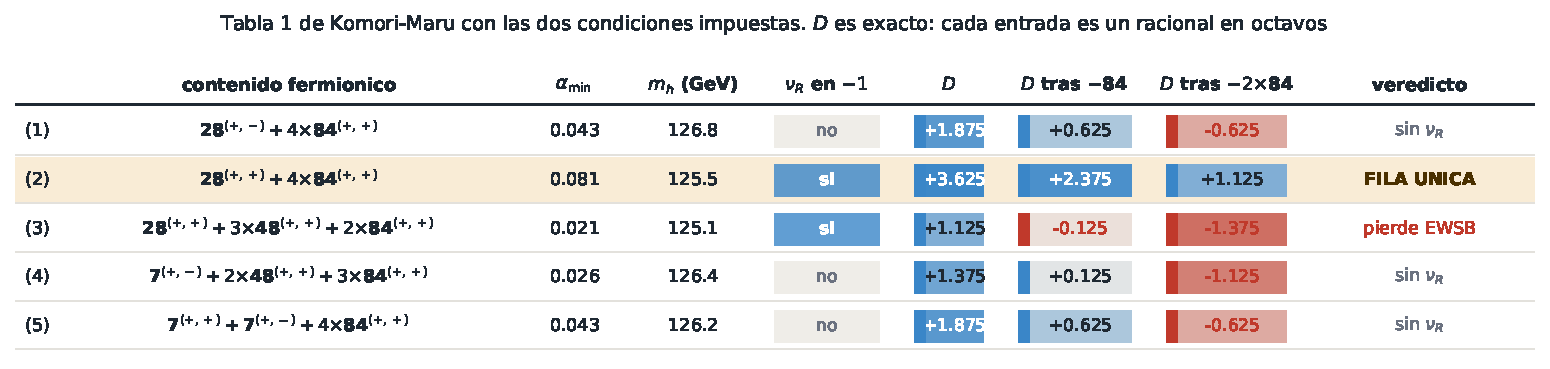
\includegraphics[width=\textwidth]{fig_table1_verdicts_es.pdf}
\caption{La Tabla~1 de \cite{KM25} con las dos condiciones de este artículo impuestas. La columna
$\nu_R$ es \S\ref{sec:anom}: qué filas contienen un singlete del Modelo Estándar de carga $U(1)'$
igual a $-1$, un enunciado sobre qué componentes existen y por tanto inmune a todo lo de
\S\ref{sec:instrument}. Las columnas $D$ son \S\ref{sec:vacuum}, antes y después de donar
$\rep{84}^{(+,+)}$ para alojar generaciones leptónicas --- una en la asignación mínima, dos en la
otra realizable; cada entrada es un racional exacto en octavos, y la barra de color lleva el signo,
que es todo el contenido. El caso (3) --- la fila que \cite{KM25} señalan como
\emph{particularmente interesante} --- solo tiene $9/8$ para gastar frente a un coste de $10/8$.
Generada por \texttt{make\_figures\_su7.py} desde el archivado
\texttt{su7\_repair\_space.json}.}
\label{fig:verdicts}
\end{figure}

Sea $\lambda$ un reescalado uniforme de todo el sector fermiónico, de modo que $\lambda=1$ es su
propia normalización, y sea $\lambda_{\rm crit}$ el valor al que una fila reducida cambia de
veredicto.

\begin{center}\small
\begin{tabular}{lrrrp{0.34\textwidth}}
\toprule
\rowcolor{hdrblue!12}
caso & $D$ suyo & $D$ tras donar un $\rep{84}$ & $\lambda_{\rm crit}$ & veredicto\\
\midrule
(1) & $15/8$ & $5/8$ & $0.8438$ & la EWSB sobrevive\\
\rowcolor{amber!12}
\textbf{(2)} & $\mathbf{29/8}$ & $\mathbf{19/8}$ & $\mathbf{0.5870}$ & \textbf{sobrevive, mayor
margen de los cinco}\\
\rowcolor{warmred!12}
\textbf{(3)} & $\mathbf{9/8}$ & $\mathbf{-1/8}$ & $\mathbf{1.0385}$ & \textbf{EWSB PERDIDA}: el
punto simétrico pasa a ser el vacío\\
(4) & $11/8$ & $1/8$ & $0.9643$ & sobrevive, por poco\\
(5) & $15/8$ & $5/8$ & $0.8438$ & la EWSB sobrevive\\
\bottomrule
\end{tabular}
\end{center}

\begin{keyeq}
\textbf{Donar un $\rep{84}$ cuesta exactamente $5/4=10/8$, y el caso (3) solo tiene $9/8$ para
gastar.} Pasa a $-1/8$, el signo cambia, y $\alpha=0$ se convierte en un mínimo genuino. Todo está
en octavos y nada es numérico.

Combinando con \S\ref{sec:anom}: solo las filas (2) y (3) pueden suministrar el $\nu_R$ requerido; de
esas, la (3) pierde la ruptura electrodébil cuando paga el escape. \textbf{El caso (2) es la única de
las cinco filas publicadas que satisface a la vez las dos condiciones necesarias --- dentro de la
extensión mínima considerada, y al nivel de la curvatura de un lazo} (Fig.~\ref{fig:verdicts}). Eso
es un filtro fuerte y no una construcción que funcione: no es la afirmación de que el caso (2)
\emph{funcione}. Es además la fila con la menor escala de compactificación de las cinco,
$1/R_5=2.0$~TeV, la más accesible. La fila que ellos destacan, el caso
(3) a $7.5$~TeV, es la que no puede.
\end{keyeq}

\noindent
\textbf{Y «merece calcularse» afirma menos de lo que parece, porque parte de ese cálculo ya existe.}
La Parte~VII \cite{PartVII} minimiza el potencial reducido y encuentra que la fila donada sin más
\emph{no} se queda dentro de la ventana original de $125$--$127$~GeV --- ninguna de las cinco lo
hace. El caso~(2) sigue siendo el banco de pruebas que este artículo selecciona porque la selección
se hace en la curvatura, donde es exacta, y porque es el más bajo de las cuatro que siguen rompiendo;
lo que falta, y lo que esa fila necesitaría para ser un modelo, es la compleción con la que termina
\S\ref{sec:open}: los términos localizados y el sector escalar. El problema siguiente no es volver a
minimizar $\rep{28}+3\times\rep{84}$: es construir la teoría alrededor del caso~(2).

\paragraph{Exacto no es lo mismo que incondicional, y la condición es una ecuación suya.} El
$3/4$ de $D$ es $\eta(3)/\zeta(3)=1-2^{1-3}$, y el $3$ es el $n^3$ de dos líneas más arriba: el
potencial va como $1/n^5$ y dos derivadas en $\alpha$ bajan un $n^2$. Ese $1/n^5$ es su ec.~(67),
demostrada en \S\ref{sec:instrument} y no supuesta aquí. Sea $w$ esa razón:
$D_i-\text{coste}$ es lineal en $w$ y el veredicto se sostiene exactamente en
$w\in[74/99,\,118/151)$. De los valores admisibles $w=1-2^{1-p}$ solo $w=3/4$ cae dentro: en $1/2$ el
caso (3) sobrevive también y la fila deja de ser única, y en $7/8$ y por encima \emph{ninguna} fila
sobrevive y la extensión mínima muere por completo. Así que la demostración de su ec.~(67) sostiene
también esta sección, no solo la \S\ref{sec:instrument}. No es una fragilidad ---$w$ está cuantizado
y sus vecinos admisibles quedan lejísimos de la ventana--- pero sí es una dependencia, y queda dicha
aquí en vez de quedar implícita.

\paragraph{Las dos condiciones son condiciones sobre la misma extensión a tres generaciones.} El
requisito de $\nu_R$ de \S\ref{sec:anom} se deriva sobre su contenido publicado de \emph{una}
generación, y la pregunta justa es si sobrevive a la extensión. Sobrevive, y por una razón que no
cuesta nada comprobar: de las catorce asignaciones solo dos caben dentro de sus propios tensores, y
ambas piden un singlete de carga $-1$ (\S\ref{sec:ladder}). Así que las dos condiciones son
condiciones sobre el mismo objeto al mismo número de generaciones --- el \emph{contenido} de bulk de
la fila debe contener un multiplete que lleve ese singlete, y debe seguir rompiendo la simetría
electrodébil una vez retirados de él los $\rep{84}^{(+,+)}$ que la asignación consume.

La segunda asignación realizable, $l=(\tfrac12,0,0)$, consume dos de ellos a un coste de $5/2$, lo
que lleva las cinco filas a $-5/8$, $9/8$, $-11/8$, $-9/8$, $-5/8$. En esa asignación el caso (2) es
la única fila que queda en pie bajo la condición del \emph{vacío} sola, antes de imponer siquiera la
condición del $\nu_R$. El caso (2) es el único superviviente en las dos.

Lo que \emph{no} afirmamos es que la carga $-1$ siguiera siendo el requisito en una teoría con más
representaciones que la suya. Las doce asignaciones descartadas arriba nombran cada una sus propias
cargas de neutrino, tomadas de $\pm\{\tfrac12,1,\tfrac32,2\}$, y solo algunas piden $-1$; quien
amplíe su contenido para alcanzar una de esas debe rehacer la primera condición. La segunda
--- el vacío --- no se ve afectada, porque $D$ no sabe para qué sirven los multipletes.

La columna $\lambda_{\rm crit}$ es el reescalado del sector fermiónico al que cada fila reducida
cambia de signo, y es la medida honesta de cuánto de esto podría comerse un error instrumental. Se
usa en \S\ref{sec:repair}, donde se generaliza de número a región.

\bridge{Un ingrediente del escape sigue sin enunciarse en su artículo: la carga del escalar que rompe
$U(1)'$. Resulta ser decidible, en forma cerrada, y es el último número libre.}

% ===================================================================
\section{La regla de selección es una semirrecta, no un ajuste fino}\label{sec:qphi}

Su modelo exige que el $U(1)'$ de \eqref{eq:u1p} se rompa mediante un escalar 4D $\varphi$ en un
punto fijo. Un valor esperado de vacío de carga $q_\varphi$ no destruye la simetría: rompe $U(1)'$
hasta un subgrupo discreto, y un operador de carga $A$ solo puede vestirse con inserciones de
$\langle\varphi\rangle$ si $A/q_\varphi\in\ZZ$. Un subgrupo residual de un $U(1)$ \emph{gauge} roto
es una simetría \emph{gauge} discreta \cite{KW,IR}, de modo que el enunciado vale a todo orden en
$\langle\varphi\rangle/M$, y queda protegido frente a los efectos que violarían una simetría
meramente global. Esa condición no es adorno: si este $U(1)'$, con sus anomalías localizadas, es
una compleción así es justo lo que \S\ref{sec:open} deja abierto. Lo que no depende de ella es el
álgebra, $A/q_\varphi\notin\ZZ$.

Su artículo no dice cuánto vale $q_\varphi$, ni qué cargas $U(1)'$ pueden vivir en un punto fijo
---coherentemente con dejar la desintegración del protón para trabajo futuro, ya que es el único
sitio donde esa carga importa. Ese único dato es el dato libre que queda para la cuestión de la regla
de selección en dimensión 6 que aquí se plantea, y es decidible en cuanto se enuncia.

Lo que el bulk fija: $\mathrm{extra}(n)=(n_6-n_7)/2$ en toda componente de todo multiplete que usan,
así que \textbf{el retículo del bulk es exactamente $\tfrac12\ZZ$}, y el $\tfrac12$ se alcanza. Un
escalar de ruptura debe ser singlete total del Modelo Estándar con $Y=0$, es decir una componente de
índice 7 puro, luego de sus propias representaciones sale
$q_\varphi\in\{\tfrac12,1,\tfrac32\}$ (el $\rep7$, el $\rep{28}$, el $\rep{84}$); el $\rep{21}$ y el
$\rep{35}$ no aportan ninguna, porque una componente de índice 7 puro necesita un índice repetido y
un tensor antisimétrico no lo tiene.

\begin{observation}[la lectura permisiva es suya, no una licencia que nos tomemos]
Tres canales de anomalía fuerzan $X_Q=-1/6$, y $-1/6$ no es múltiplo de $1/2$. Así que, a falta de un
mecanismo de Green--Schwarz, su propia consistencia obliga a la lectura \emph{permisiva} de lo que
puede vivir en un punto fijo --- y la lectura permisiva es precisamente la que pone el punto
peligroso $A=0$ al alcance. Su construcción ya la usa: la razón que dan para localizar los quarks, en
la frase anterior a su ec.~(47), es que las hipercargas fraccionarias de los quarks no salen de
productos tensoriales de $\rep7$. Un campo de brana suyo lleva ya, por tanto, una carga fuera del
retículo del bulk --- la hipercarga --- y $X_Q$ hereda exactamente esa libertad.
\end{observation}

\begin{proposition}[la regla en forma cerrada]\label{prop:closed}
La protección falla en $q_\varphi$ si y solo si $q_\varphi=|A_j|/n$ para alguna generación $j$ y
algún entero $n\ge1$. Ese conjunto es numerable y tiene \emph{máximo}, luego la protección es una
semirrecta.
\end{proposition}

\emph{Control:} la forma cerrada se contrastó con un barrido exhaustivo de todo racional $p/q\le2$
con $q\le36$, para las 14 soluciones --- $18\,648$ valores, \textbf{0 discrepancias}. De ahí salen
cotas y no ajustes finos: la asignación mínima $l=(\tfrac12,\tfrac12,0)$, con
$A=(\tfrac16,\tfrac16,-\tfrac13)$, falla exactamente sobre $\{1/(3n)\}$ y está protegida para
\emph{todo} $q_\varphi>1/3$ --- más fino que nada de su espectro, de modo que sus tres valores la
protegen. La única asignación de las catorce compatible con la lectura estricta,
$l=(\tfrac12,\tfrac12,-1)$ con $X_Q=0$, falla en $q_\varphi=\tfrac12$ y en $q_\varphi=1$, y solo el
$\tfrac32$ del $\rep{84}$ la protege --- pero pide el peldaño $3$, un tensor de cinco cajas que su
contenido no tiene.

\begin{keyeq}
\textbf{Así que ninguna asignación es a la vez compatible con la lectura estricta y realizable dentro
de sus propios tensores.} Las dos que caben están en $X_Q=-1/9$ y $-1/18$, ninguna sobre el retículo
del bulk $\tfrac12\ZZ$; la que sí está sobre el retículo no se puede construir. Bajo la lectura
estricta, su modelo no tiene extensión a tres generaciones dentro de su propio contenido --- lo que
obliga a la lectura permisiva por segunda vez, y con un argumento independiente del $X_Q=-1/6$ de una
generación de más arriba.
\end{keyeq}

Encender Green--Schwarz --- el escape que mantiene viva la lectura estricta --- libera $X_Q$ a $m/2$,
luego $A=(3m+1)/2$, que nunca es cero. Entonces $A/q_\varphi$ en $q_\varphi=3/2$ vale $(3m+1)/3$, que
nunca es entero porque $3m+1$ nunca es divisible por $3$. Aquí el grupo residual es $\ZZ_3$
---$q_\varphi$ es el triple del cuanto del retículo--- y esa divisibilidad \emph{es} el enunciado de
que los cuatro operadores están cargados bajo él, así que la regla y el grupo son un solo hecho y no
dos. \textbf{El nombre del grupo es relativo a una normalización y la regla no lo es.} $\ZZ_3$ es el
residual \emph{sobre el retículo estricto de semienteros}, donde $\tfrac12$ es el cuanto global y
$q_\varphi=3/2$ son tres de ellos. En la rama permisiva las cargas de brana $-1/9$ y $-1/18$ son
estados del mismo $U(1)'$, luego el cuanto global es más fino, ese mismo $q_\varphi$ genera un grupo
cíclico mayor, y el residual solo puede nombrarse después de fijar la normalización global. Lo que no
se mueve es $A/q_\varphi\notin\ZZ$, que es toda la regla de selección:

\begin{keyeq}
\textbf{$q_\varphi=3/2$ --- la carga de la componente $(777)$ de un $\rep{84}$, el multiplete que
todas las filas de su Tabla~1 ya contienen --- prohíbe los cuatro operadores de dimensión 6 con
$|\Delta B|=1$ a todo orden en $\langle\varphi\rangle/M$, para toda carga semientera del quark de
brana, sin dependencia de familia y sin hipótesis alguna sobre las anomalías.}

\smallskip
\noindent\emph{Léase con sus precondiciones, que no son adorno.} «A todo orden» es a todo orden en la
inserción, y vale para: \emph{un} escalar de ruptura --- con varios el grupo residual es
$\gcd(q_1,q_2,\dots)$, y dentro de su propio contenido \emph{toda} pareja de las tres cargas
disponibles tiene $\gcd=\tfrac12$, de modo que \emph{cualquier} segundo escalar que condense destruye
exactamente esta protección; una
normalización global fija de la carga; ningún campo adicional cuya carga encoja el subgrupo residual;
y los cuatro operadores enumerados en \S\ref{sec:anom}, no toda la base de operadores de dimensión
superior. Lo que el modelo todavía no tiene es un sector escalar explícito que explique por qué rompe
en esta dirección y no en otra.
\end{keyeq}

\emph{Controles que tenían que saltar, o el enunciado estaría vacío:} $q_\varphi=\tfrac12$ falla para
\emph{todo} $m$ y $q_\varphi=1$ para todo $m$ impar. Ninguno de los dos es vacío, de modo que $3/2$
discrimina de verdad y no es un universal trivial. Estructuralmente, un escalar cuya carga \emph{es}
el cuanto del retículo deja como grupo residual $\ZZ_1$; la protección necesita que $q_\varphi$ sea
múltiplo \emph{propio} del cuanto. Y un ataque acabó generando una hipótesis en vez de confirmar
otra: con dos escalares de ruptura el grupo residual lo genera $\gcd(q_1,q_2)$, y como las tres
cargas que su contenido ofrece son $\tfrac12,1,\tfrac32$, las tres parejas tienen $\gcd=\tfrac12$ y
hunden el grupo residual hasta $\ZZ_1$. Así que no es que una añadidura concreta tenga mala suerte:
el escalar del $\rep{84}$ tiene que ser el \emph{único} que condense. El caso de un
solo escalar es por tanto la cota optimista, y queda escrito en vez de supuesto.

\bridge{Todo lo anterior es un signo, un racional exacto o una forma cerrada, y ni una línea es un
número en GeV. Fue deliberado. ¿Qué le pasa al instrumento para que hiciera falta?}

% ===================================================================
\section{El instrumento, y dónde falla}\label{sec:instrument}

No reproducimos la columna $\amin$ de su Tabla~1 a partir de sus fórmulas publicadas. Nuestros
mínimos son $0.0553$, $0.0831$, $0.0436$, $0.0469$, $0.0553$ frente a sus $0.043$, $0.081$, $0.021$,
$0.026$, $0.043$ --- cocientes $1.29$, $1.03$, $2.08$, $1.80$, $1.29$. Esta sección enuncia qué ha
quedado excluido, porque son las exclusiones las que hacen la discrepancia informativa y no
simplemente incómoda.

\textbf{No es el sector gauge.} Su ec.~(68) se reconstruye exactamente desde su ec.~(62): los
coeficientes $\{2,4,7\}$ salen de un recuento sobre los mismos ocho multipletes, con el $7$ desglosado
como $4+3$, y sin que entre ningún fantasma. Eso solo contrasta su álgebra contra una ecuación suya
anterior; \S\ref{sec:setting} cierra el hueco derivando esos mismos tres coeficientes de la tabla
$(q,P_5P_5',P_6)$ del adjunto, de modo que el sector gauge queda ahora excluido al mismo nivel que el
fermiónico y no apoyado en su propia aritmética. Su ec.~(67) queda probada: sumando su ec.~(66) y
combinando con $+2/(\pi n)^6$, el $-8$ cancela el $+32/16$ exactamente y toda la llave se cierra en
$\tfrac{3k}{4(\pi n)^5}\big[P_6+g(\pi kn)\big]$ con
$g(x)=\coth x+x\,\mathrm{csch}^2x+\tfrac23x^2\coth x\,\mathrm{csch}^2x$, $g(\infty)=1$, y Sage
simplifica la diferencia a exactamente $0$.

\textbf{No es la truncación $k\gg1$.} De esa forma cerrada, la corrección es exponencialmente pequeña
en $k$: $1.5\%$ en $k=1.2$, $0.02\%$ en $k=2$, y $O(1)$ solo para $k\lesssim0.5$ --- el régimen
\emph{opuesto} al suyo. No puede mover $\amin$ en absoluto. \emph{Una nota anterior nuestra que decía
que esta reparación ``necesita $k\approx1.2$'' queda retractada: ese número nunca se calculó. Lo
imprimía como cadena literal en cada fila un bucle que solo ajustaba otros dos parámetros.}

\textbf{No es la transcripción.} Sus ecs.~(73)--(76) se verifican por tres vías independientes: a
mano desde $s=\eta\eta'$; por recuento de multipletes $\su2_L$ contra las descomposiciones (41),
(57), (69), (70); y contando directamente componentes de la línea de Wilson real, ya que su ec.~(77)
es la identidad salvo en los índices 5 y 7, de modo que el argumento del coseno de una componente es
$|n_5-n_7|\pi n\alpha$ y su signo es $P_5P_5'$ --- teoría de grupos pura, independiente de sus
ecuaciones. Las cuatro representaciones reproducen nuestra tabla de términos exactamente. El recuento
confirma además, por su cuenta, la regla que enuncian en una sola frase tras su ec.~(71) y no vuelven
a usar: el $\rep{84}$ tiene $24$ estados en $(1,-1)$, es decir $12$ términos $=$ los $11$ que listan
más el autovalor menor del cuadruplete. Prescindir de esa regla triplica un $\chi^2$ de contraste
($419.7$ frente a $102.3$), luego hace falta. El mismo recuento encuentra lo que parece una errata, y
vale la pena pasarla porque la corrección es de un carácter: los quince
dobletes del $\rep{84}$ solo salen si los dos términos impresos con subíndice $\rep{48}$ en su
ec.~(76) son términos del $\rep{84}$.

\textbf{No es multiplicativa.} Su ec.~(80) da una segunda columna calculada, y es una restricción
fuerte que no se había usado. Con $V=CF$, $C=3k/(64\pi^8R_5^6)$, tanto $R_6$ como $k=R_5/R_6$ se
cancelan idénticamente, y su ec.~(82) elimina $R_5$; lo que queda tiene que ser independiente de la
fila:
\begin{keyeq}
\begin{equation}\label{eq:K}
K\;\equiv\;\frac{m_h\,\amin}{\sqrt{F''(\amin)}}\;=\;2m_W\,g_4\sqrt{\frac{3}{16\pi^6}}\;=\;2.245624\,g_4 .
\end{equation}
\emph{Un invariante de todo modelo cuya masa de Higgs sea su ec.~(80), cuya masa del $W$ sea su
ec.~(81), y cuyo potencial lleve un prefactor independiente de la fila --- verificado simbólicamente,
y que hasta donde sabemos no se había escrito antes.} Las dos primeras son suyas; la tercera es lo
que lo convierte en un test y no en una definición, y \S\ref{sec:setting} muestra que la segunda está
forzada en su modelo en vez de tomada prestada del de cinco dimensiones.
\end{keyeq}
Escribiendo $F=G+\sum_R w_R f_R$ con $G$ la parte gauge (exacta), la estacionariedad en sus
$\alpha_i$ y su $m_h$ vía las ecs.~(80),(82) son \emph{ambas lineales} en
$(w_7,w_{28},w_{48},w_{84},1/g_4^2)$: diez ecuaciones, cinco incógnitas, sin optimizador y sin mínimo
local. La columna $\amin$ \emph{sola} es satisfacible ($\|\mathrm{res}\|=0.0064$, y pide
$w(\rep{48})=5.59$); añadir las cinco ecuaciones de $m_h$ la rompe ($0.1628$). Su tabla está dada a
dos cifras significativas, así que el residuo tiene un suelo: muestreando $300$ puntos de la caja de
redondeo ($\pm0.0005$ en $\alpha$, $\pm0.05$~GeV en $m_h$) sale un \emph{mínimo} de $0.1580$ y una
mediana de $0.1635$. El redondeo no lo explica. Una reponderación por canal sí ajusta ($0.0031$) ---
y la rechaza su propio control, que ajusta igual de bien datos permutados ($0.0030$, cociente
$0.97$), y el que necesite $g_4=2.39$ frente al valor $0.63$ del Modelo Estándar.

\begin{figure}[t]
\centering
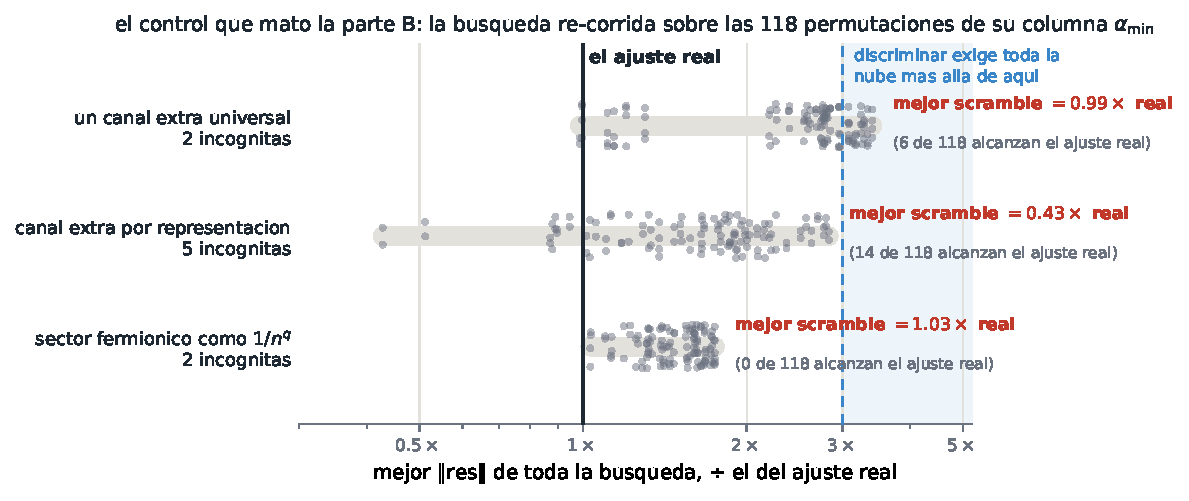
\includegraphics[width=\textwidth]{fig_anchor_controls_es.pdf}
\caption{El control que decide la última exclusión de \S\ref{sec:instrument}. Cada reparación
candidata es un barrido --- un canal extra $v\sum_n s^n\cos(c\pi n\alpha)/n^p$ sobre $c\in[0.5,40]$,
$p\in\{3,\dots,7\}$, $s=\pm1$, o el sector fermiónico como $1/n^q$ --- de modo que el control tiene
que rehacer el \emph{barrido entero} sobre datos permutados, y no volver a resolver en los parámetros
ganadores. Puntos grises: el mejor residuo de la búsqueda completa en cada una de las $118$
permutaciones no triviales de su propia columna $\amin$, dividido por el del ajuste real. Para
discriminar haría falta que toda la nube quedara más allá del umbral discontinuo; en cambio, cada
nube monta sobre $1$, y en dos de los tres tests los datos permutados \emph{ganan} a los reales.
Generada por \texttt{make\_figures\_su7.py}.}
\label{fig:controls}
\end{figure}

\textbf{Y no es un canal extra.} Los tres candidatos que quedaban --- un argumento del coseno fuera de
$\{1,2,3\}\times\pi n\alpha$, una dependencia en $n$ que no sea $1/n^5$, o multipletes que no estén en
(69),(70) --- son un mismo objeto, $\delta(\alpha)=v\sum_n s^n\cos(c\pi n\alpha)/n^p$, y el sistema
sigue siendo lineal. Barrer $(c,p,s)$ y rehacer el barrido entero sobre las $118$ permutaciones de su
columna $\amin$ (Fig.~\ref{fig:controls}) da mejores permutados de $0.99\times$ y $0.43\times$ el
ajuste real, y $51$ de los $80$ valores de $c$ caen a menos de $3\times$ del ganador: un bosque, no un
mínimo. La variante $1/n^q$ necesita el sector fermiónico $15\times$ más débil que su propia
ec.~(72).

\textbf{Y su propia tabla no es una errata.} Su ec.~(82) hace de la tercera columna de la Tabla~1 una
función de la primera, $1/R_5=2\times80.4~\text{GeV}/\amin$, y habíamos usado las dos primeras
durante tres días sin comprobarla. Las cinco filas son consistentes: cada par impreso
$(\amin,1/R_5)$ tiene un intervalo común no vacío a dos cifras significativas. Así que la
discrepancia es sobre el potencial y no sobre un número mal tecleado --- una posibilidad que no se
había cerrado nunca. En las filas (3) y (4), las dos que fallan todo lo demás, la columna $1/R_5$ es
de hecho la restricción \emph{más afilada} sobre $\amin$, al $20\%$ y al $35\%$ de la anchura
ingenua; intersecar las cajas mueve el residuo mínimo solo de $0.1561$ a $0.1563$, así que compra
precisión y ninguna exclusión nueva.

\textbf{Y el instrumento no está roto en general.} Toda exclusión anterior es interna a este cálculo.
La pregunta externa --- si un potencial de línea de Wilson a un lazo ensamblado de este modo
reproduce siquiera un vacío gauge-Higgs \emph{publicado} --- se responde en la Parte~V de esta serie,
contra un artículo $\su4$ en 6D con un autor en común \cite{AHMN}: el vacío sale exacto,
$(0.438,0.299)$ frente a $(0.438,0.299)$, y el cociente de masas del Higgs al $0.1\%$. Aquella
comparación se hizo sobre cocientes, de modo que era ciega a lo único que una discrepancia en $\amin$
podría ser: una mala normalización global. No lo es: sus tres elementos publicados de la matriz de
masas se encuentran con los nuestros a través de una \emph{única} constante con una dispersión del
$0.54\%$, y esa constante es $1/4\pi^7$, el prefactor de su propia ec.~(4.1), que no fue ningún dato
de entrada nuestro. Su $\lambda_{\min}$ sale entonces $0.058799$ frente a su $0.058791$. Esa es una
implementación distinta --- la de la Parte~V se construye con caracteres de Schur sobre dos fases de
Wilson, esta cuenta componentes de una sola --- así que no demuestra que el ensamblaje $\su7$ sea
correcto. Demuestra que el método reproduce un vacío 6D publicado \emph{y su escala absoluta}, lo que
saca la normalización global de la lista de cosas que podría ser el fallo del ancla.

\begin{observation}[la lista de exclusiones anterior es la lista de UN lazo, y no es todo el espacio]
\label{obs:looporder}
Todo lo excluido en esta sección vive a un lazo, y los tres candidatos estructurales nombrados arriba
son los candidatos de un lazo. Hay un cuarto: el \emph{orden de lazos}. El potencial de línea de
Wilson es el potencial del lazo de Polyakov de la teoría gauge térmica, donde el cálculo a dos lazos
es antiguo. A dos lazos en gauge puro es un reescalado multiplicativo e independiente del fondo del
resultado a un lazo, $\Omega^{(2)}/\Omega^{(1)}=-5g^2C_2(A)/(16\pi^2)$ para cualquier grupo clásico o
excepcional \cite{DGKA} --- lo que aquí ya está excluido, porque la $\lambda$ que pide la columna
$\amin$ no es un solo número. Con fermiones esa proporcionalidad falla \cite{GuoDu}, y las
expresiones llevan polinomios de Bernoulli de los ángulos de fondo individuales \emph{y de sus
diferencias por pares}. Esos ángulos son las cargas de línea de Wilson, de modo que un producto de
dos de esas estructuras genera cosenos en $c_b\pm c_d$: con $c\in\{1,2,3\}$ eso alcanza
$c\in\{0,\dots,6\}$, y $4,5,6$ caen fuera del conjunto. Numéricamente $5g^2C_2(A)/(16\pi^2)$ vale
$7$--$14\%$ para $g_4\in[0.55,0.80]$ con $C_2(A)=7$, frente al reescalado del $4$--$20\%$ que pide la
columna $\amin$: \emph{el mismo orden}. No hemos calculado ese término para este modelo y nada de lo
que hay aquí depende de él; lo que establece es que la lista anterior es la lista de un lazo. Tampoco
rescata la Tabla~1, ya que su potencial, su $m_h$ y la finitud que motiva la unificación gauge-Higgs
son todos enunciados a un lazo. La pregunta acotada que deja es teórico-de-grupos y no necesita
ninguna integral de lazo, y la respondemos: \emph{¿depende el potencial fermiónico a dos lazos de la
representación solo a través del multiconjunto de sus cargas?} No. Con
$\mathrm{Tr}(T^aT^b)=\delta^{ab}/2$, su peso es exactamente $2\sum_a|T^a_{ij}|^2$ en la fundamental,
de modo que el reemplazo para $R$ general está forzado a ser
$W(w,w')=\sum_a|\langle w|T^a_R|w'\rangle|^2$, cuyas sumas por fila son $C_2(R)$; y
$\rep{48}^{(+)}$ frente a $4\times\rep7^{(+)}+\rep7^{(-)}+\rep{28}^{(+)}$ tienen tablas de términos a
un lazo idénticas --- luego $F$, $\amin$, $m_h$ y $D$ idénticos --- con $\sum C_2$ de $7$ frente a
$24.8571$. El potencial a un lazo es ciego a los estados de carga cero, así que fija el índice de
Dynkin y no el Casimir. Ninguno de los dos miembros de ese par es un contenido de la Tabla~1, luego
nada de lo publicado aquí queda separado por él.
\end{observation}

\begin{observation}[el guarda mintió primero, y queda registrado]
La primera versión de ese control era la habitual de este programa: fijar $(c,p,s)$ en el ganador,
invertir la columna $\amin$ y volver a resolver. Devuelve cocientes $3.41$ y $3.51$ y el veredicto
``informativo'' sobre tests que están muertos. Barrer es en sí mismo una búsqueda, de modo que un
control que no rehace la búsqueda no mide nada. Tanto el guarda roto como su arreglo están en la
salida archivada.
\end{observation}

Un diagnóstico merece reportarse porque es afilado y no sabemos dónde colocarlo. En su $\alpha$
publicada, las filas (1), (2) y (5) satisfacen el invariante de $m_h$ con nuestra $F''$ \emph{sin
modificar} en $g_4=0.60322$, $0.61847$ y $0.59943$, cerca del valor $0.63$ del $\su2_L$ del Modelo
Estándar; la fila (4) se desvía en un factor 3; y la fila (3) --- la que ellos destacan y dibujan en
su Fig.~2 --- tiene $F''(0.021)=-2.44883317179876457187207506193<0$, exacto, de modo que su ec.~(80)
no devuelve allí masa de Higgs real alguna. El potencial no se vuelve convexo hasta
$\alpha=0.0238002801693$, que es $1.133\times$ su $\amin$. El valor exacto sale de una forma cerrada
que merece anotarse por sí misma: todo término del potencial es
$\mathrm{Re}\,\mathrm{Li}_5\!\left(s\,e^{ic\pi\alpha}\right)$, luego
\[
F(\alpha)=\sum_{\text{términos}}m\,\mathrm{Re}\,\mathrm{Li}_5\!\left(s\,e^{ic\pi\alpha}\right),
\qquad
F''(\alpha)=-\sum_{\text{términos}}m\,(c\pi)^2\,\mathrm{Re}\,\mathrm{Li}_3\!\left(s\,e^{ic\pi\alpha}\right),
\]
sin truncación alguna --- lo que importa, porque $F''$ es la serie $1/n^3$, de convergencia lenta.

\paragraph{Dónde vive el residuo, con el confundido dicho en la misma frase.} Las dos filas que
fallan son exactamente las dos cuyo contenido lleva un $\rep{48}$ --- la (3) con $3\times\rep{48}$,
la (4) con $2\times\rep{48}$ --- y el único sistema lineal que la columna $\amin$ \emph{sí} satisface
pide $w(\rep{48})=5.59$, la mayor reponderación individual de toda esta sección. Ese número merece la
barra de error que nunca ha llevado, porque el $\rep{48}$ es aquí la coordenada mal condicionada: es
el $99\%$ de la dirección singular más blanda de la matriz de diseño, con un valor singular $75$
veces menor que el más rígido. Sobrevive de todos modos. El perfil del residuo tiene allí un mínimo
genuino y no una meseta, y propagar el único ruido que estos datos tienen --- sus dos cifras
significativas --- da $w(\rep{48})\in[5.20,6.00]$ al $95\%$, una anchura relativa del $14\%$ frente
al $1\%$ de $w(\rep{84})$, y sigue excluyendo el $1$ por un factor cinco. Una dirección blanda solo
está mal medida en relación con el ruido, y aquí el ruido son dos decimales de una tabla. Dos
instrumentos que no comparten aritmética apuntan al mismo multiplete, es decir a su ec.~(75). El
confundido va al lado: esas dos filas son también exactamente las dos de menor $\amin$, y con cinco
filas las dos lecturas no se pueden separar. Lo que las separaría es una sexta fila publicada --- un
contenido con $\rep{48}$ y $\amin$ grande, o uno sin $\rep{48}$ y pequeño --- y no existe tal verdad
publicada.

Podría existir, sin embargo, y eso conviene fijarlo en vez de dejarlo como lamento. De los $427$
contenidos que rompen la simetría electrodébil entre los seis fermiones que su propio texto permite,
$22$ caen en $120$--$132$~GeV, una banda en torno a su propia ventana de selección; y dentro de esa
banda los dos rangos de $\amin$ \emph{se solapan}, $[0.0180,0.0734]$ con $\rep{48}$ frente a
$[0.0288,0.0873]$ sin él. El candado entre las dos lecturas es, por tanto, un accidente de las cinco
filas que eligieron, y no una propiedad del modelo. El rompedor más limpio es
$\rep{28}^{(+,-)}+\rep{28}^{(+,+)}+\rep{48}^{(+,+)}+3\times\rep{84}^{(+,+)}$, que nosotros situamos
en $\amin=0.0734$ y $m_h=126.2$~GeV --- dentro de su propia ventana de $125$--$127$, y con un
$\rep{48}$ a un $\amin$ mayor que el de cualquier fila con $\rep{48}$ que imprimieran.

\begin{keyeq}
\textbf{Así que la predicción puede escribirse antes de que la fila exista.} En sus cinco filas,
$\amin^{\rm nuestro}/\amin^{\rm suyo}$ vale $1.94$ donde hay un $\rep{48}$ y $1.20$ donde no lo hay.
Para ese contenido, las dos lecturas se comprometen por tanto a números distintos: un $\amin$
publicado cerca de $0.0378$ si el locus es el $\rep{48}$, y cerca de $0.0612$ si lo es el $\amin$
pequeño. Difieren en un factor $1.62$, que dos cifras significativas resuelven. No adoptamos ninguna,
y dejamos anotadas las dos.
\end{keyeq}

\noindent
En contra de la lectura del $\rep{48}$: su ec.~(75) está transcrita correctamente por partida doble,
a mano desde $s=\eta\eta'$ y por un recuento independiente de estados sobre el $\su2$ generado por
$T^{44}$, dando ambos las multiplicidades $1,2,8$. De modo que \emph{si} el $\rep{48}$ es el locus,
lo que está mal no es nuestra lectura de su ecuación --- y esa es una afirmación sobre el artículo de
otro que cinco datos no sostienen y que no hacemos. Queda anotada porque convierte «no conseguimos
reproducir la Tabla~1» en una pregunta con dirección.

\begin{keyeq}
Esto se enuncia como \textbf{una pregunta para los autores y no como una afirmación de defecto}. Tres
controles independientes de transcripción pasan, de modo que un residuo que no sabemos colocar es más
probablemente nuestro que suyo; \S\ref{sec:scope} enuncia el alcance que eso deja. La pregunta tiene
lugar y testigo: \emph{¿qué ingrediente de su \S3.2 lleva de las ecs.~(68) y (72)--(76) al $\amin$ de
la Tabla~1?}
\end{keyeq}

\bridge{Un instrumento abierto solo es fatal si la conclusión depende de él. ¿Cuánto del instrumento
toca de verdad un veredicto que es el signo de un solo número racional?}

% ===================================================================
\section{Por qué la discrepancia no alcanza a la conclusión}\label{sec:repair}

La objeción honesta a \S\ref{sec:vacuum} es que $D$ se calcula precisamente con las ecuaciones que
fallan en \S\ref{sec:instrument}. La respondemos no en un punto sino sobre una región: tratamos el
residuo como una reponderación desconocida por representación $w_R$ --- la deformación
\emph{multiplicativa} más general, y la familia que contiene toda reparación que los datos hayan
pedido jamás --- y preguntamos para qué $w$ sobrevive la conclusión.

$D$ es exactamente lineal en $w$, y los coeficientes por multiplete son la tabla de
\S\ref{sec:vacuum}. De ahí se siguen dos cosas de inmediato.

\begin{keyeq}
\textbf{(i) $D(\rep{48}^{(+,+)})=0$ idénticamente en $w(\rep{48})$.} El $\rep{48}$ aporta
$mc^2=1\cdot4+2\cdot1=6$ en $s=+1$ y $8\cdot1=8$ en $s=-1$, y $6-\tfrac34\cdot8=0$. El monomio está
\emph{ausente} del polinomio, no es pequeño en él. Así que $w(\rep{48})=5.59$ --- la mayor reparación
individual que pide la columna $\amin$, y el único sistema lineal que los datos del ancla \emph{sí}
satisfacen --- es invisible a la conclusión. No aproximadamente: idénticamente.


\textbf{(ii) La conclusión es la cuña}
\[
2\,w(\rep{28})+\tfrac54\,w(\rep{84})\;<\;\tfrac{27}{8}\;<\;2\,w(\rep{28})+\tfrac{15}{4}\,w(\rep{84}),
\]
siendo la desigualdad izquierda «la fila (3) muere» y la derecha «la fila (2) vive». No aparece ni
$w(\rep7)$ ni $w(\rep{48})$: la conclusión vive en un plano.
\end{keyeq}

\paragraph{Ese mismo cero hace el papel contrario en \S\ref{sec:ladder}, y conviene decirlo sin
rodeos.} Aquí $D(\rep{48})=0$ es lo que hace la conclusión \emph{robusta}: el peso peor ajustado del
artículo no puede tocarla. Allí es lo que la hace \emph{precaria}: un $\rep{48}$ donado gratis no le
costaría nada al caso (3), y el caso (3) tiene tres. Un número, dos papeles, ninguna contradicción
---el primero trata de repesar un multiplete que se queda en el potencial, el segundo de sacar uno
de él.

\begin{figure}[t]
\centering
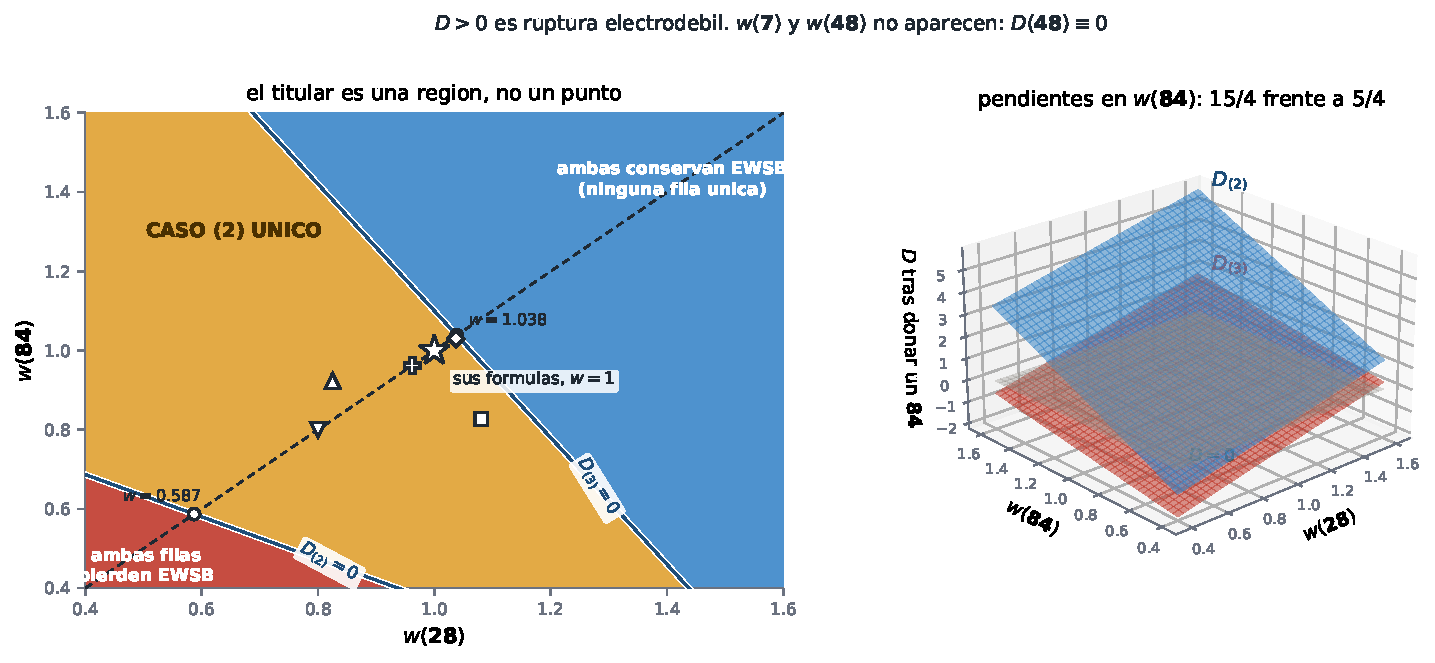
\includegraphics[width=\textwidth]{fig_repair_space_es.pdf}
\caption{\textbf{Izquierda:} el plano $(w(\rep{28}),w(\rep{84}))$, coloreado por veredicto tras donar
un $\rep{84}^{(+,+)}$. La región ámbar es donde el caso (2) sobrevive y el (3) no --- la conclusión
de este artículo. Las marcas huecas son todas las reparaciones a las que se ha ajustado alguna vez la
discrepancia del ancla (\S\ref{sec:instrument}); todas caen dentro, y $w=1$ también. La diagonal
discontinua lleva el intervalo $(27/46,\,27/26)=(0.587,\,1.038)$, que reproduce los
$\lambda_{\rm crit}$ de \S\ref{sec:vacuum} por otra vía. \textbf{Derecha:} por qué es una cuña ---
$D$ para las dos filas son dos planos sobre el mismo cuadrado, con pendientes $15/4$ y $5/4$ en
$w(\rep{84})$, y la conclusión es la losa entre sus conjuntos de ceros. Generada por
\texttt{make\_figures\_su7.py}.}
\label{fig:repair}
\end{figure}

Como $D_{(2)}-D_{(3)}=\tfrac52\,w(\rep{84})>0$ para cualquier peso positivo, la fila (3) no puede
sobrevivir nunca a la (2); el plano tiene tres regiones y no cuatro. Cortado a lo largo de
$w(\rep{28})=w(\rep{84})=w$, las fronteras son los racionales exactos $27/46=0.5870$ y
$27/26=1.0385$, que son precisamente los $\lambda_{\rm crit}$ de \S\ref{sec:vacuum} alcanzados por
una vía independiente. \textbf{La conclusión se sostiene en todo el intervalo
$w\in(0.5870,1.0385)$, un factor $1.77$ de anchura, y ese intervalo contiene $w=1$.} Toda reparación
jamás ajustada cae dentro de la cuña (Fig.~\ref{fig:repair}); el margen más fino es el del sistema de
curvatura sola, en $w(\rep{84})=1.030$ frente a un techo de $1.0385$, y ese sistema está exactamente
determinado y por tanto no dice nada --- pero es donde un lector escéptico debe apretar, y lo decimos
en vez de suavizarlo.

La reponderación por canal de \S\ref{sec:instrument} muere aquí por tercera vez, y en un instrumento
que nunca ve $\amin$ ni $m_h$: con los pesos por canal que ajustan ($0.13$--$0.28$, donde su ec.~(72)
dice $1$), las cinco filas tienen $D<0$ --- \emph{ninguna ruptura electrodébil en absoluto},
incluidas las filas cuyos números publicados el ajuste se construyó para reproducir. Una reparación
que reproduce dos números de una fila destruyendo el fenómeno que esa fila existe para exhibir no es
una reparación.

Por último, toda la \S\ref{sec:vacuum} se reconstruyó solo desde teoría de grupos, sin consultar en
ningún momento sus ecs.~(73)--(76): desde la base de cargas de línea de Wilson $u,v=(5\pm7)/\sqrt2$ y
la paridad por índice $\pi=P_5P_5'=(+,+,+,-,-,+,-)$, las descomposiciones
$\rep{28}=\mathrm{Sym}^2(\rep7)$, $\rep{84}=\mathrm{Sym}^3(\rep7)$ y
$\rep{48}=\rep7\otimes\rep{\bar7}-\rep1$ reproducen cada multiplicidad de término, cada $D$ por
multiplete, y las dos fronteras $27/46$ y $27/26$, simbólicamente en
$\mathbb{Q}[w_7,w_{28},w_{48},w_{84}]$. Allí el $\rep{28}$ se construye como
$\mathrm{Sym}^2(\rep7)$ y no como la conjugada identificada en \S\ref{sec:setting}, y eso no es
inconsistencia: la conjugación invierte el signo de toda carga y deja intactas todas las paridades,
mientras que $D$ ve la carga solo a través de $c=2|q|$ con los estados ya emparejados como $\pm q$.
Las dos lecturas dan el mismo $D$ término a término. Esa construcción no aplica en ningún momento la
regla del $(1,\rep4)$ de su ec.~(71) --- el autovalor menor del cuadruplete es sin más una componente
de $\mathrm{Sym}^3(\rep7)$ con carga $1/2$, contada como cualquier otra --- y aterriza igualmente en
el mismo $12$, lo que confirma su regla de una frase desde el otro lado.

\paragraph{La cuña es un enunciado de un lazo, y es más fina justo donde está la pregunta abierta.}
El coeficiente gauge $27/8$ se mantiene fijo arriba, y a un lazo eso es correcto: la parte gauge se
reconstruye y no se ajusta, y \S\ref{sec:setting} la deriva de la propia tabla de carga y paridad del
adjunto en vez de desde su ec.~(62) --- lo que importa aquí y en ningún otro sitio, porque este es el
único peso que la cuña no deja flotar. Solo entra el \emph{cociente} del peso fermiónico al peso
gauge, y la cuña dice que está en $(27/46,\,27/26)$. Los dos márgenes desde $1$ no son simétricos:
$19/46=41.304\%$ por debajo, y $1/26=3.846\%$ por encima. Equivalentemente --- y esta es la forma que
importa --- suprimir solo el sector gauge en más de $1/27=3.7037\%$ hace que la fila (3) sobreviva
también a la donación, y el caso (2) deja de ser único. Un reescalado común a los dos sectores no
cambia nada en absoluto, lo cual se asevera en vez de suponerse.

Ese umbral debe leerse frente a la Observación~\ref{obs:looporder}. El único candidato al ingrediente
que falta que este artículo no puede excluir es el orden de lazos, y un término de dos lazos no
respeta la partición: en gauge puro multiplica el sector gauge por $1-5g^2C_2(A)/(16\pi^2)$, que con
$C_2(A)=7$ vale $6.70$--$14.19\%$ sobre $g_4\in[0.55,0.80]$, mientras que con fermiones se sabe que
la proporcionalidad falla \cite{GuoDu}. Eso es entre $1.8$ y $3.8$ veces el margen.

\paragraph{Y esa estimación es demasiado gruesa, en la dirección que importa.} Lee la alarma de la
supresión \emph{sólo gauge}, pero el sector fermiónico también se suprime, y cuánto está publicado en
el mismo sitio: la ec.~(5.13) de \cite{GuoDu} da
$\Gamma^{(2)}_f/\Gamma^{(1)}_f=-3g^2C_F(N)/(8\pi^2)$ frente al $-5g^2C_2(A)/(16\pi^2)$ de
\cite{DGKA}, de modo que
\[
  \frac{\delta_f}{\delta_b}=\underbrace{\frac{6}{5}}_{\text{integrales 4D}}\cdot
  \underbrace{\frac{C_F}{C_2(A)}}_{\text{teoría de grupos}}
  =\frac{3(N^2-1)}{5N^2}=\frac{144}{245}=0.5878 \quad\text{en } N=7 .
\]
Los dos factores hay que mantenerlos separados, y sólo el segundo transfiere: el $6/5$ es
$(3/8)\big/(5/16)$, un cociente de coeficientes de lazo \emph{cuadridimensionales}. La teoría de
grupos sola da $C_F/C_2(A)=(N^2-1)/2N^2<1/2$, así que haría falta un cociente de coeficientes por
encima de $2N^2/(N^2-1)\simeq2.04$ para que el sector fermiónico fuese el más suprimido y $w$ bajase;
en cuatro dimensiones ese cociente es $1.2$. La conclusión de que \textbf{$w$ sube} es por tanto
\emph{robusta} --- sobrevive a un factor $1.7$ de error en los coeficientes transplantados --- pero
no es un teorema, y no se enuncia como tal. Sólo el tamaño depende de $g_4$.

Corregida para la mitad fermiónica, el equivalente gauge-solo del efecto neto,
$1/(1-s)=(1+\delta_f)/(1+\delta_b)$, vale $2.88\%$ en $g_4=0.55$ y $6.38\%$ en $g_4=0.80$: no
$1.8$--$3.8$ veces el margen sino $0.78$--$1.72$, cruzándolo en $g_4=0.6205$. Al $g_4=0.63$ que usa
esta serie se sienta en $1.033$ veces --- \emph{por encima del techo, un $0.13\%$}. Calculado en
\texttt{twoloop\_wedge.py}, con el control de que un reescalado común a los dos sectores devuelve
exactamente $1$.

Dicho así suena a alarma, y un borrador anterior la contestaba con los datos del ancla: $\amin$ es
monótona creciente en el peso fermiónico en las cinco filas y la nuestra es demasiado \emph{grande}
en las cinco, de modo que la reponderación que pide la columna $\amin$ es una \emph{supresión} del
sector fermiónico, y resolver $\arg\min F=\amin^{\rm suyo}$ fila a fila da $0.8483$, $0.9619$,
$0.8102$, $0.7996$, $0.8480$ --- todas dentro de la cuña y todas \emph{por debajo} de $1$
(\texttt{su7\_\allowbreak wedge\_\allowbreak direction.py}, cuya salida archivada los sigue llevando).

\textbf{Esa respuesta queda retirada, y la razón vale más que la respuesta.} Esos cinco números son
un \emph{ajuste}, no una medida de $w$. Dicen qué reponderación uniforme reproduciría cada fila
\emph{por separado}, y una reponderación uniforme daría un número: dan cinco, repartidos en un $20\%$
de $0.7996$ a $0.9619$. Un residuo que no es uniforme no es una reponderación, y la Part~VII
compañera lo localiza en otro sitio --- su segunda ancla publicada valida el potencial y el
minimizador, y deja el diccionario específico del modelo como lo que queda por explicar. Una paridad
o una carga mal asignadas cambian el potencial término a término, que es exactamente cómo se dispersa
un ajuste a eso. Los cinco números miden el tamaño de esa discrepancia en unidades de peso, fila a
fila, y no llevan información sobre dónde está el $w$ físico.

\begin{figure}[htbp]
\centering
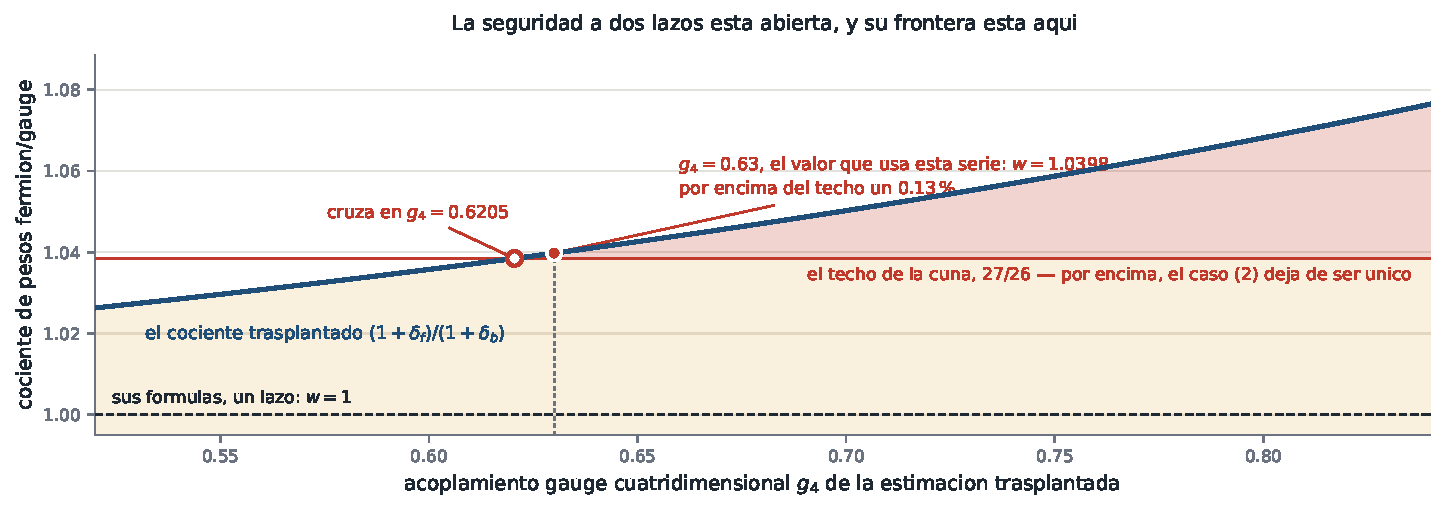
\includegraphics[width=\textwidth]{fig_ratio_line_es.pdf}
\caption{Dónde está la frontera de validez del veredicto de este artículo. El veredicto es un
enunciado sobre un solo número, el cociente de pesos fermión/gauge $w$; \S\ref{sec:repair} muestra que
se sostiene sobre la cuña, cuyo techo es $27/26$ (rojo). Lo que la cuña no absorbe es el orden de
lazos, así que la curva es el cociente de dos lazos trasplantado $(1+\delta_f)/(1+\delta_b)$,
construido con la mitad gauge de \cite{DGKA} y la fermiónica de \cite{GuoDu}, frente al acoplamiento
cuatridimensional de esos resultados. Cruza el techo en $g_4=0.6205$, y al $g_4=0.63$ que usa esta
serie queda un $0.13\%$ por encima: del lado \emph{malo}, y por menos de medio por ciento.
\textbf{No dibujadas, y a propósito: las cinco reponderaciones fila a fila que pide la columna
$\amin$.} Son un ajuste y no una medida de $w$, el argumento que las usaba queda retirado en la
página anterior, y una figura no puede seguir sosteniendo un argumento que el texto ha retractado.
Dibujada por \texttt{make\_figures\_su7.py} desde el archivado \texttt{twoloop\_wedge.json}.}
\label{fig:ratio}
\end{figure}

Quitado el ajuste, se cae la defensa. A un lazo $w=1$ por construcción, ya que el sector gauge se
reconstruye y no se ajusta; y la estimación de arriba pone el transplante de dos lazos en $1.0398$
frente al techo de $1.0385$. \textbf{Nada en los datos del ancla empuja de vuelta, y el borrador
anterior decía que sí.} Lo que los datos del ancla sí dicen es lo que \S\ref{sec:instrument} ya
afirma de ellos: la discrepancia es real, está sin explicar, y vive en el diccionario y no en la
maquinaria.

\begin{keyeq}
\textbf{La seguridad a dos lazos está abierta, y aquí es donde está la frontera de validez.} El
veredicto es robusto frente a toda la familia de deformaciones multiplicativas de un lazo: la cuña
$(27/46,\,27/26)$ contiene $w=1$ y toda reparación jamás ajustada a la discrepancia. \textbf{Un
término de dos lazos no tiene por qué pertenecer a esa familia} --- no está obligado a ser un
reescalado uniforme de nada (\S\ref{sec:open}), de modo que puede no existir un $w$ efectivo que
mover. El análogo publicado más cercano, cuatridimensional y térmico en sus dos mitades, pone el
cociente trasplantado en $1.0398$ frente al techo $1.0385$: del lado peligroso, al acoplamiento
nominal, por menos de medio por ciento, y cruza en $g_4=0.6205$ (Fig.~\ref{fig:ratio}). Ese
trasplante no zanja la pregunta en seis dimensiones y
aquí no se pretende que lo haga. Lo que sí hace es localizar la frontera exactamente.
\end{keyeq}

\noindent
De modo que la exposición se enuncia a su tamaño real y del lado por el que realmente cae, en vez de
argumentarse hasta hacerla desaparecer. Este artículo tenía un argumento de que caía del lado
seguro, y ese argumento es justo el retirado más arriba: leía una dirección en cinco ajustes fila a
fila, y cinco ajustes que se dispersan un $20\%$ miden la discrepancia y no el peso. Lo que
zanjaría la pregunta es el cálculo en seis dimensiones que nadie ha hecho. Su mitad acotada de teoría
de grupos no necesita integral de lazo y se contesta aquí ---Observación~\ref{obs:looporder} y las
dos primeras entradas de \S\ref{sec:open}---: dos lazos sí ve contenido que uno no puede ver, luego
el cociente no puede suponerse igual a $1$.

\bridge{Todo paso anterior tomó prestado un mecanismo de alguien. El último trabajo del argumento es
decir de quién, y dónde termina el préstamo.}

% ===================================================================
\section{Atribución}\label{sec:scope}

\textbf{Todo mecanismo empleado aquí es de otro}, y las puertas siguientes se corrieron antes de
escribir los resultados correspondientes, no después.

% un longtable, no un tabular: como caja inquebrantable ocupaba casi una pagina y
% no cabia bajo su propio encabezado, dejandolo varado con 312 pt de blanco
\begingroup\small
\begin{longtable}{p{0.55\textwidth}p{0.38\textwidth}}
\toprule
\rowcolor{hdrblue!12}
mecanismo & estado\\
\midrule
\endfirsthead
\toprule
\rowcolor{hdrblue!12}
mecanismo & estado\\
\midrule
\endhead
las extensiones $U(1)$ del Modelo Estándar libres de anomalías son
$\mathrm{span}\{Y,B-L\}$, y un $B-L$ gaugeado necesita neutrinos dextrógiros de carga $-1$ &
de manual, y de hace cuarenta años\\
un $B-L$ gaugeado no logra prohibir los operadores de protón que conservan $B-L$; la cura es un
$B-x_iL$ dependiente de familia & \cite{FamilyU1}, literal en su resumen; el enunciado de
dimensión 6 es de Weinberg y de Wilczek--Zee \cite{Weinberg,WZ}\\
situar las familias en representaciones distintas o en puntos fijos distintos de una GUT de
orbifold, y suprimir así la desintegración del protón & construcción de modelos GUT de orbifold
estándar \cite{Raby,OrbGUT}\\
un $U(1)$ adicional roto deja una simetría \emph{gauge discreta} residual capaz de prohibir los
operadores de protón de dimensión 4, 5 y 6 & \cite{KW,IR,DiscGauge,Orth}\\
las anomalías localizadas restringen las cargas de brana, y Green--Schwarz puede absorber las mixtas
de $U(1)$ & von Gersdorff--Quir\'os; Kojima--Takenaga--Yamashita \cite{KTY}, que \cite{KM25} citan
como su ref.~[13]\\
los campos de brana en GUT de orbifold no tienen por qué formar representaciones heredadas del bulk &
práctica estándar; es por lo que sus propios quarks pueden estar localizados siquiera\\
la materia en la adjunta ---una representación real--- es vectorial, y lo que la vuelve quiral es una
proyección $\ZZ_3$ & \cite{GMN}, literal en su introducción: \emph{``It is well known that\dots\ The
matter in the adjoint representation is always vector-like, but one can project out the vector-like
partner by a $Z_3$ transformation.''} La Proposición~\ref{prop:real} es la especialización a sus
paridades diagonales $\pm1$, donde esa cura no está disponible; los recuentos y los controles
quirales sí son nuestros\\
un $U(1)$ sobrante en unificación gauge-Higgs roto por un escalar con valor esperado de vacío de
orden $1/R$, con la carga superviviente leída de la dirección de ese valor & \cite{GHK},
ecs.~(50)--(54), (77), (79) --- el mecanismo de \S\ref{sec:qphi} es suyo\\
no hay Yukawa local de brana para los leptones cargados en unificación gauge-Higgs, y la obstrucción
se califica de genérica & \cite{SSS,Maru19} --- pertinente al cierre peldaño a peldaño del Yukawa de
\S\ref{sec:ladder}, y por eso ese cierre es un control y no un resultado\\
\rowcolor{amber!13}
una regla práctica que selecciona el contenido fermiónico por la curvatura del potencial de línea de
Wilson \emph{en el origen} & \cite{AdachiMaru}. Es el antecedente más cercano a \S\ref{sec:vacuum}:
su hessiano factoriza en $\alpha=0$ y su regla de selección es nuestra aritmética --- \textbf{en el
origen, y solo ahí}. Lo que no es suyo es el racional exacto $D$ por multiplete, y el coste de la
donación que de él se sigue\\
minimalidad más cancelación de anomalías fijando el contenido de familias del Modelo Estándar &
\cite{GengMarshak} --- trasfondo de \S\ref{sec:anom}, que es un enunciado relativo dentro de un
modelo fijo y no una clasificación\\
\bottomrule
\end{longtable}
\endgroup

\textbf{Lo nuestro} es la especialización a su modelo: que sus propias ecs.~(43)--(47) y (76)--(79)
fuerzan $U(1)'=T_{3L}+Y-(B-L)$ y por tanto ninguna protección a una generación; que su espectro exige
un neutrino dextrógiro de carga $-1$ que solo el $\rep{28}$ suministra --- y que es exigido y no
meramente suficiente --- y que solo las filas (2) y (3) lo contienen; la escalera de peldaños dentro
de su $\su7$, la identidad de la Proposición~\ref{prop:identity}, las catorce asignaciones
supervivientes junto con las dos que sus propios tensores pueden alojar, y que el $\rep{84}^{(+,+)}$
que aloja el peldaño 1 ya está en todas las filas de su Tabla~1; la forma cerrada
$V''(0)=-\pi^2\zeta(3)D$ con su tabla racional por multiplete, y la selección del caso (2) como única
fila publicada que sobrevive a las dos condiciones; la regla de selección en forma cerrada
$q_\varphi=|A_j|/n$ con su máximo, y
$q_\varphi=3/2$ como protector universal por un argumento módulo 3; el invariante $K$ de
\S\ref{sec:instrument}; y el resultado de región de \S\ref{sec:repair}.

\textbf{Lo que no se afirma.}
\emph{Ningún $\amin$, $1/R_5$ ni $m_h$ para contenido modificado alguno} --- el instrumento de
\S\ref{sec:instrument} lo prohíbe, y todo lo anterior se enuncia como un signo, un racional exacto o
una forma cerrada precisamente por eso. \emph{Que el caso (2) funcione}: lo que se muestra es que es
el único candidato que queda; hacerlo funcionar es cálculo suyo tanto como nuestro, y si una fila
superviviente sigue cayendo en $m_h=125$--$127$~GeV no se responde aquí. \textbf{Queda así una
pregunta que sí podemos enunciar con precisión y no podemos contestar aquí: tras la donación,
¿sigue la fila superviviente dentro de $125$--$127$~GeV?} Contestarla exige minimizar el potencial
modificado, que exige una forma cerrada para $\amin$ que este artículo no tiene; Part~VII
\cite{PartVII} la aporta y la contesta.
\emph{Ningún valor esperado de vacío, escala, coeficiente ni vida media} --- \S\ref{sec:qphi} es una
regla de selección, no una predicción de $\tau_p$. \emph{Operadores por encima de dimensión 6}, cuyas
cargas no se enumeraron. \emph{Que más de un escalar no rompa $U(1)'$} --- con varios, el grupo
residual lo fija $\gcd(q_1,q_2,\dots)$, lo que solo puede dificultar la protección.
\emph{Que las anomalías mixtas de $U(1)$ tengan que cancelar sobre materia localizada} ---
Green--Schwarz sigue disponible, y encenderlo hace el resultado de \S\ref{sec:qphi} más fuerte y no
más débil, que es la dirección poco habitual. \emph{Que la discrepancia del ancla sea suya} --- tres
controles pasan, así que un residuo que no sabemos colocar es más probablemente nuestro. \emph{Y
ningún defecto en su artículo en ninguna parte de este trabajo}: lo que \S\ref{sec:instrument}
reporta es una pregunta abierta, y lo que \S\ref{sec:setting} reporta sobre el $\rep{28}$ y sobre
$\pi_5=\pi_7$ son datos no enunciados con consecuencias calculadas.

Su artículo tiene \emph{una} generación --- las palabras \emph{generación} y \emph{familia} no
aparecen en él fuera del título de una referencia --- de modo que de \S\ref{sec:ladder} en adelante
se habla de la extensión a tres generaciones que su modelo tendrá que tener y todavía no tiene.
Conseguir tres generaciones es de por sí un problema no enunciado en su artículo; el escape vive
exactamente dentro de él.

\bridge{Eso es lo que hace el artículo, y de quién es cada mecanismo. Antes de preguntar qué deja
abierto, conviene poner en una página cada afirmación que sí hace, con el control que la sostiene
---incluidos los dos controles que volvieron diciendo \emph{no comprobada}.}

% ===================================================================
\section{Verificación}\label{sec:verif}

Toda afirmación de más arriba se reúne aquí una vez, contra la evidencia que la sostiene. Donde
un enunciado está demostrado, la entrada es la demostración y el control sobre su
implementación; donde sólo está medido, la entrada lo dice, y donde un control pudo saltar y no
saltó, también. \textbf{Una afirmación cuyo control pasa también sobre datos barajados queda
registrada como no comprobada, no como confirmada} --- dos lo están, y son las dos que merecen
leerse dos veces. Los dos últimos bloques son por donde debería empezar un referee: lo que está
\emph{abierto}, y lo que un borrador anterior afirmaba y éste retira.

\begingroup
\small
\begin{longtable}{p{0.62\textwidth}p{0.31\textwidth}}
\caption{Cada afirmación de este artículo contra la evidencia que la sostiene. Los bloques son, por
orden: lo que se afirma; lo que se reporta como \emph{dato} de \cite{KM25} y no como defecto; lo que
queda \emph{abierto}; y lo que un borrador anterior afirmaba y este retira.}\\
\toprule
\rowcolor{hdrblue!12}
\textbf{Afirmación} & \textbf{Dónde, y sobre qué}\\
\midrule
\endfirsthead
\toprule
\rowcolor{hdrblue!12}
\textbf{Afirmación} & \textbf{Dónde, y sobre qué}\\
\midrule
\endhead
Tres canales de anomalía fuerzan $X_Q=-1/6$, que es exactamente $A=0$ & \S\ref{sec:anom}; seis
canales, rederivados independientemente en Sage desde el anillo de caracteres de $A_6$\\
$U(1)'=T_{3L}+Y-(B-L)$ sobre todo campo, y los cuatro operadores tienen $Y=B-L=0$ &
\S\ref{sec:anom}, una identidad\\
Dos canales no pueden cancelar y exigen un singlete de carga $-1$; existe en el $\rep{28}$ y en
ningún otro sitio, luego solo las filas (2),(3) lo suministran & \S\ref{sec:anom}; $\sum x=-1$ y
$\sum x^3=-1$ son independientes\\
Un $\rep{28}$ es \emph{necesario} y no meramente mínimo: el conjunto de soluciones es $e=-1-4w$,
$u=5w$, luego el número neto de $\rep{28}$ nunca es cero & \S\ref{sec:anom}; y un barrido por fuerza
bruta sin $\rep{28}$ no devuelve nada, mientras que el mismo barrido quitando una condición sí
devuelve soluciones\\
Solo dos de las catorce asignaciones caben dentro de sus propios tensores, y ambas exigen carga
$-1$ & \S\ref{sec:ladder}; el peldaño $\ge2$ no es alojable ---cuatro cajas para las potencias
tensoriales, y para el $\rep{48}$, que no lo es, ningún modo cero quiral. Las catorce se
rederivan con una implementación independiente\\
\rowcolor{amber!12}Proposición~\ref{prop:real} ---el mecanismo es de \cite{GMN}, la especialización
nuestra---: con sus paridades diagonales $\pm1$ una representación real no da ninguna generación
quiral, luego el $\rep{48}$ no puede alojar el escape ---y un $\rep{48}^{(+,+)}$
habría costado $D=0$ exactamente & \S\ref{sec:ladder}, demostrada en tres líneas y contada en
\texttt{su7\_adjoint\_is\_vectorlike.py}, con el $\rep{28}$ y
el $\rep{84}$ como control que tiene que salir quiral y sale ($10$ y $34$ estados sin emparejar). El
caso (3) tiene tres $\rep{48}$, así que esto es un paso y no un inciso\\
Su ec.~(81), citada para el modelo $\su4$ en 5D, está forzada por su propia ec.~(54): el $W$ lleva
carga de línea de Wilson $\tfrac12$ y el fotón $0$ & \S\ref{sec:setting}; los modos de carga $1$
existen, así que el control no es vacío\\
$\mathrm{extra}(L)=(1-k)/2$, y $\mathrm{extra}(L)+\mathrm{extra}(e^c)=1/2$ en todo peldaño &
\S\ref{sec:ladder}; el peldaño 0 devuelve su propia ec.~(43)\\
Proposición~\ref{prop:identity}: $[\su2_L]^2U(1)'=\tfrac12\sum_jA_j$ & \S\ref{sec:ladder}, exacta;
14 asignaciones sobreviven a los seis canales\\
El peldaño 1 lo aloja un $\rep{84}^{(+,+)}$, que está en todas las filas de la Tabla~1; el
$\rep{35}$ no puede alojarlo & \S\ref{sec:ladder}, desde sus ecs.~(37)--(40)\\
$V''(0)=-\pi^2\zeta(3)D$, $D$ racional; $\rep{48}^{(+,+)}\mapsto0$, $\rep{84}^{(+,+)}\mapsto5/4$ &
\S\ref{sec:vacuum}; el residuo de truncación se \emph{predice} al $2\%$\\
\rowcolor{amber!12}\textbf{El caso (2) es la única de las cinco filas publicadas que suministra el
$\nu_R$ y sobrevive a la donación --- dentro de la extensión mínima, y a curvatura de un lazo} &
\S\ref{sec:anom} $+$ \S\ref{sec:vacuum}, Fig.~\ref{fig:verdicts}; todo en octavos. Un banco de
pruebas seleccionado, no un modelo entregado: no se recalcula el potencial modificado.
\emph{Depende de su ec.~(67)}: el veredicto se sostiene en $w\in[74/99,118/151)$ y solo $w=3/4$ es
admisible ahí\\
Proposición~\ref{prop:closed}: la protección falla si y solo si $q_\varphi=|A_j|/n$; el conjunto
tiene máximo & \S\ref{sec:qphi}; $18\,648$ valores de barrido exhaustivo, $0$ discrepancias\\
$q_\varphi=3/2$ prohíbe los cuatro operadores a todo orden para todo $X_Q$ semientero &
\S\ref{sec:qphi}; y $q_\varphi=1/2$ y $1$ fallan ambos, luego no es vacío\\
$K=m_h\amin/\sqrt{F''(\amin)}$ es independiente de la fila, cancelándose $R_5,R_6,k$ &
\S\ref{sec:instrument}, verificado simbólicamente\\
$D(\rep{48})\equiv0$, y la conclusión es una cuña que contiene $w=1$ y toda reparación ajustada &
\S\ref{sec:repair}, Fig.~\ref{fig:repair}; reconstruido desde teoría de grupos en Sage\\
Sus términos con subíndice $\rep{48}$ en la ec.~(76) tienen que ser términos del $\rep{84}$,
identificado por un recuento & \S\ref{sec:instrument}; los quince dobletes del $\rep{84}$ solo salen
así\\
$F=\sum m\,\mathrm{Re}\,\mathrm{Li}_5(s\,e^{ic\pi\alpha})$ y $F''$ una suma de
$\mathrm{Re}\,\mathrm{Li}_3$, sin truncación & \S\ref{sec:instrument}, verificado en Sage; es lo que
hace exacto el $F''(0.021)$ de $30$ dígitos\\
Sus ecs.~(54),(41),(57),(69),(70) y su espectro KK están derivados, no supuestos, y no hay nada mal
en ellos & \S\ref{sec:setting}; $13/13$ constantes de estructura, la omitida exactamente cero, cargas
$\{0,\pm\tfrac12,\pm1\}$ con multiplicidades $26,20,2$\\
Su ec.~(68) también: sus tres coeficientes se siguen de la tabla $(q,P_5P_5',P_6)$ del adjunto con
dos pesos, $a=2$ y $b=\tfrac12$ & \S\ref{sec:setting}; sobredeterminado, y las dos filas que fijan
$a$ coinciden. Este es el sector que la cuña mantiene fijo, y era el único contrastado contra nada
más que su propia ec.~(62)\\
\midrule
\rowcolor{hdrblue!10}\textbf{No enunciado en su artículo, reportado como dato y no como defecto} &
\textbf{Dónde}\\
\midrule
Su $\rep{28}$ es $\mathrm{Sym}^2(\rep{\bar7})$, la conjugada & \S\ref{sec:setting}; $4/4$ frente a
$2/4$, y el test discrimina ($\rep{84}$: $10/10$ frente a $1/10$). Invisible a $V_{\rm eff}$\\
$\pi_5=\pi_7$: los dos índices que la línea de Wilson mezcla llevan el mismo $P_5P_5'$, sin lo cual
su ec.~(72) no está bien definida & \S\ref{sec:setting}, \S\ref{sec:repair}; lo primero que comprueba
la construcción en Sage\\
Su espectro exige un neutrino dextrógiro, no enunciado en su artículo & \S\ref{sec:anom}\\
Su Tabla~1 es internamente consistente: la ec.~(82) hace de $1/R_5$ una función de $\amin$, y los
cinco pares impresos concuerdan & \S\ref{sec:instrument}; un control sobre \emph{su} tabla que podía
haber saltado. En las filas (3),(4) la columna $1/R_5$ es la restricción más afilada\\
\midrule
\rowcolor{hdrblue!10}\textbf{Abierto, y enunciado como abierto} & \textbf{Por qué}\\
\midrule
El $\amin$ de su Tabla~1 no se reproduce desde sus ecs.~(68),(72)--(76) & \S\ref{sec:instrument};
sector gauge exacto, truncación irrelevante, transcripción verificada por tres vías, y ninguna
reparación multiplicativa ni de canal único sobrevive a su propio control\\
El caso (3) tiene $F''<0$ en su propio $\amin$ publicado bajo nuestro ensamblaje &
\S\ref{sec:instrument}; exacto a 30 dígitos, y la inflexión está en $1.133\times$ ese valor\\
\rowcolor{hdrblue!7}\textbf{La lista de exclusiones anterior es la lista de \emph{un lazo}} &
\S\ref{sec:instrument}, Observación~\ref{obs:looporder}. Dos lazos en gauge puro es multiplicativo y
por tanto ya está excluido; con fermiones no lo es, y su tamaño es del mismo orden que el reescalado
que pide la columna $\amin$. No calculado aquí, y así dicho\\
\rowcolor{warmred!12}\textbf{Y la cuña también}: tolera $1/27$ de reescalado relativo
gauge-frente-a-fermión, y los reescalados de dos lazos publicados ponen el transplante
\emph{por encima} al acoplo nominal &
\S\ref{sec:repair}. Con la mitad fermiónica de \cite{GuoDu} incluida, $0.78$--$1.72$ veces el margen
sobre $g_4\in[0.55,0.80]$ ---no el $1.8$--$3.8$ de una lectura sólo gauge---, cruzando en
$g_4=0.6205$ y en $1.033$ al $g_4=0.63$. Un borrador anterior lo contestaba con la columna del
ancla; esa respuesta queda \textbf{retirada}\\
\rowcolor{warmred!12}\textbf{Y los dos inputs de esa estimación son cuadridimensionales y térmicos} &
sus factores de grupo son esta álgebra, sus integrales de lazo no, y el $6/5$ está hecho de las
segundas. \cite{DGKA} añaden una limitación propia, en sus palabras: no han \emph{``succeeded in
finding a general proof''} de su ec.~(66) que evite la evaluación explícita, y no saben cómo funciona
la combinatoria \emph{dentro} de la cámara de Weyl --- su prueba cubre los caminos rectos del origen
a los mínimos $Z(N)$, por las aristas. Un $\amin\simeq0.05$ no está en ninguno de los dos\\
Las dos filas que fallan son exactamente las dos que contienen un $\rep{48}$, y el único sistema
satisfacible pide $w(\rep{48})=5.59$, $[5.20,6.00]$ al $95\%$ bajo su propio redondeo &
\S\ref{sec:instrument}; confundido con que sean las dos de menor $\amin$, y cinco filas no pueden
separar las lecturas. Su ec.~(75) está verificada por partida doble, luego no se afirma defecto
alguno\\
El instrumento está validado solo \emph{como método} & \S\ref{sec:instrument}: la implementación
independiente de la Parte~V reproduce \cite{AHMN} exactamente, pero es otra implementación, así que
no certifica el ensamblaje $\su7$\\
\midrule
\rowcolor{warmred!14}\textbf{Retractado, y dejado a la vista} & \textbf{Por qué}\\
\midrule
``las ecs.~(62)--(65) exactas necesitan $k\approx1.2$'' & nunca se calculó; una línea de conclusión
impresa como cadena literal. La corrección real es del $1.5\%$ en $k=1.2$. \S\ref{sec:instrument}\\
``un canal extra repara el ancla, y el control dice que es informativo'' & el control fijaba el
ganador en vez de rehacer la búsqueda. \S\ref{sec:instrument}, Fig.~\ref{fig:controls}\\
\bottomrule
\end{longtable}
\endgroup

\bridge{Leído ese libro mayor, los puntos abiertos son las filas sin demostración y sin medida. ¿Qué
necesita cada uno, y cuáles puede el propio instrumento de este artículo volver ya lo bastante
precisos como para entregárselos a alguien?}

% ===================================================================
\section{Problemas abiertos}\label{sec:open}

\S\ref{sec:verif} registró lo que se sostiene. Esta es la otra lista: lo que el trabajo
\emph{abre}. Cada entrada nombra la magnitud que la decide, el umbral que esa magnitud debe cruzar y
el test que la zanjaría ---una pregunta sin test que discrimine es un estado de ánimo y no un
problema--- y cada una dice a qué línea de trabajo pertenece, porque en todos los casos el linaje es
lo que vuelve la pregunta precisa en vez de simplemente sin contestar. Van en el orden en que cada
una entrega a la siguiente sus datos.

\paragraph{1. ¿El término fermiónico a dos lazos sube el cociente fermión/gauge, o lo baja?} Ese
único signo decide \S\ref{sec:repair}: subirlo más allá de $27/26$ cuesta el veredicto, bajarlo no
cuesta nada y además explicaría el ancla. Ahora son dos márgenes y no uno, y son independientes: la
cuña de \S\ref{sec:repair} mide cuánto puede moverse el \emph{peso de un multiplete}, y la ventana
$w\in[74/99,118/151)$ de \S\ref{sec:vacuum} mide cuánto puede moverse la \emph{razón alternante}. Un
término a dos lazos no tiene por qué respetar ninguno de los dos ---no está obligado a ser un
reescalado uniforme de nada---, así que se citan los dos, y un cálculo que caiga fuera de cualquiera
de ellos cambia la respuesta. La mitad teórico-de-grupos ya está hecha, y ya dice esto: el factor de
materia a dos lazos \emph{no} queda determinado por el multiconjunto de cargas de un lazo.
El peso que sustituye al de \cite{GuoDu} para una representación general está forzado a ser
$W(w,w')=\sum_a|\langle w|T^a_R|w'\rangle|^2$, cuyas sumas por fila son $C_2(R)$, y \emph{no} es
función del multiconjunto de cargas --- de modo que un término de dos lazos ve contenido que uno solo
no puede ver, y el cociente no puede suponerse igual a $1$. Lo que falta son las integrales de lazo
en seis dimensiones, adonde la estructura de Bernoulli del cálculo térmico en cuatro nunca se ha
llevado. Esa laguna no la nombramos nosotros: el potencial de línea de Wilson a dos lazos en
unificación gauge-Higgs se ha calculado una vez, en \cite{HMTY} ---con un autor de
\cite{AdachiMaru} entre ellos--- para QED en $M^4\times S^1$, y su propia introducción dice por qué
se detuvo ahí: \emph{``Evaluation of the Higgs mass at the two loop level is formidable in
non-Abelian gauge theory. To get insight in the problem it is instructive to examine, as the first
step, QED on $M^4\times S^1$.''} Diecinueve años después, el caso no abeliano con representación
general sigue siendo la continuación de ese primer paso.
El observable que separa los dos órdenes de lazo existe y está exhibido: $\rep{48}^{(+)}$
frente a $4\times\rep7^{(+)}+\rep7^{(-)}+\rep{28}^{(+)}$ tienen tablas de términos a un lazo
idénticas --- luego $F$, $\amin$, $m_h$ y $D$ idénticos --- y $\sum C_2$ de $7$ frente a $24.8571$.
\emph{Nuestra, y lo más duro de aquí.}

\paragraph{1b. Y hasta dónde llega ese ``ve más'', que está acotado --- y la cota tampoco necesita
integral de lazo.} La respuesta de arriba es un negativo sin techo: dos lazos ven contenido que uno
no ve, y nada decía cuánto más. Lo que sí puede decirse, y contando en vez de calculando, es qué
\emph{clase} de dato de representación le está permitido usar a un segundo lazo:

\begin{quote}
\textbf{a dos lazos no puede aparecer ninguna traza de materia de orden superior a cuadrático}, de
modo que lo que el segundo lazo añade es \emph{dato cuadrático resuelto por cargas} y no un
invariante de Casimir de orden superior.
\end{quote}

\noindent
Eso es un enunciado sobre el orden de la traza, no una clasificación de topologías de dos lazos, y
la diferencia importa más abajo.

Escríbase el factor de grupo dependiente del contenido de un diagrama de vacío a dos lazos como una
traza sobre la representación. El factor \emph{sunset} $\sum_a\mathrm{tr}_R(T^a f(H) T^a g(H))$ se
reduce, clase de raíz a clase de raíz, a cinco tablas de una \emph{sola} carga, porque para una raíz
con $\Delta=\langle\alpha,T\rangle$ fija la segunda carga queda determinada:
\[
  N_\Delta(q)\;=\!\!\sum_{w:\,q_w=q}\ \sum_{\alpha:\,\langle\alpha,T\rangle=\Delta}
  \bigl|\langle w+\alpha|E^\alpha|w\rangle\bigr|^2 ,
\]
y dos contenidos dan el mismo \emph{sunset} \emph{cualesquiera que sean las integrales de lazo}
exactamente cuando sus cinco tablas coinciden --- las integrales son factor común y se cancelan en la
comparación. Su suma no necesita ni un elemento de matriz: de
$C_2=\sum_i H_i^2+\sum_\alpha E^\alpha E^{-\alpha}$ sale
$\sum_\Delta N_\Delta(q)=\sum_{w:q_w=q}\mathrm{mult}(w)[C_2(R)-|w|^2]$.

Queda el ingrediente que \cite{HMTY} nombran como su propia frontera --- \emph{``there appear a new
interaction vertex proportional to $H$''} --- y se zanja contando en vez de calculando. Para un grafo
de vacío conexo $2I=\sum_k kV_k$, luego
\[
  L \;=\; I-V+1 \;=\; 1+\tfrac12\sum_k V_k\,(k-2),
\]
y el número de lazos depende de las \emph{valencias} y de nada más. Una pata de fondo es un campo
clásico externo: $k$ cuenta las patas \emph{cuánticas} que entran en un vértice una vez insertado el
fondo, de modo que una pata de fondo no aporta media arista interna y no puede cambiar $I$ ni $V$,
aunque sí cambia el tensor del vértice. Así, una inserción en una línea de materia y un vértice
de tres gluones con una pata de fondo pesan ambos cero: pueden añadirse sin límite y no cambian nada.
Escribiendo $a$ para los vértices cúbicos materia-gauge y $b$ para los \emph{seagull}, el orden de la
traza de materia sobre un lazo es $a+2b$, y a dos lazos $a+2b\le a+2b+c+2d+g=2$. \textbf{Una traza
cúbica exige $a+2b\ge3$, luego peso $\ge3$, luego $L\ge3$: ningún diagrama de dos lazos puede
llevarla.} Figura~\ref{fig:twoloop}. El fondo tampoco puede aportar el índice adjunto que falta,
siendo una dirección de Cartan fija.

De modo que los dos enunciados son complementarios y no rivales. Dos lazos sí ven contenido que uno
no puede --- ése es el par de arriba, y por eso el cociente no puede suponerse --- pero lo que ven
sigue siendo cuadrático en los generadores cuánticos, resuelto por las cargas del fondo: las tablas
$N_\Delta(q)$, y ningún invariante de orden superior.

\textbf{Lo que esto no es, dicho antes de que lo pregunte un referee.} El conteo de valencias acota
el \emph{orden} de la traza de materia sobre un lazo. No es una enumeración de topologías de dos
lazos, y no quedan aquí clasificados: los diagramas con más de un lazo de materia, las distintas
contracciones de índices adjuntos entre ellos, los contratérminos y las contribuciones localizadas
en seis dimensiones, y las estructuras de vértice no abelianas más allá de la que \cite{HMTY}
nombran. Dos contenidos que coincidan en las cinco tablas coinciden por tanto en el factor sunset y
en todo factor de grupo de dos lazos construido a partir de una sola traza de materia ---que es
hasta donde llega el conteo--- y no en el potencial de dos lazos entero. Dentro de ese alcance la
conclusión es la útil: \emph{una degeneración que sobrevive a $C_2$ no está esperando a que un
Casimir de orden superior la levante.}

Lo que el conteo no aporta es el número del que depende la entrada~1. Acota la \emph{clase} de dato
de representación que un segundo lazo puede usar; el signo de $\delta_f/\delta_b-1$ sigue
necesitando las integrales en seis dimensiones. Y los datos publicados tampoco lo aportan: cinco
filas y un solo cociente libre, con las dos filas que fallan compartiendo a la vez un $\rep{48}$ y
los dos $\amin$ más pequeños. Esa degeneración en los datos es la entrada siguiente.

\begin{figure}[htbp]
\centering
\begin{tikzpicture}[
  every node/.style={font=\scriptsize},
  matter/.style={draw=hdrblue!80,thick},
  gauge/.style={draw=warmred!75,thick,decorate,
                decoration={coil,aspect=0,segment length=1.7mm,amplitude=0.55mm}},
  bg/.style={-{Latex[length=1.6mm]},okgreen!80,thick},
  lbl/.style={font=\scriptsize,align=center}]
\def\R{6.5mm}
\begin{scope}[xshift=0mm]
  \draw[matter] (0,0) circle (\R);
  \draw[gauge] (-\R,0) -- (\R,0);
  \node[lbl] at (0,-11mm) {\emph{sunset}\\ $a=2$,\ orden $2$};
\end{scope}
\begin{scope}[xshift=26mm]
  \draw[matter] (-6mm,0) circle (4.6mm);
  \draw[matter] (6mm,0) circle (4.6mm);
  \draw[gauge] (-1.4mm,0) -- (1.4mm,0);
  \node[lbl] at (0,-11mm) {burbuja doble\\ $a=2$,\ orden $1$};
\end{scope}
\begin{scope}[xshift=52mm]
  \draw[matter] (0,0) circle (\R);
  \draw[gauge] (0,\R) .. controls (5mm,13mm) and (-5mm,13mm) .. (0,\R);
  \node[lbl] at (0,-11mm) {\emph{seagull}\\ $b=1$,\ orden $2$};
\end{scope}
\begin{scope}[xshift=78mm]
  \draw[matter] (0,0) circle (\R);
  \coordinate (v) at (0,12mm);
  \draw[gauge] (-4.6mm,4.6mm) -- (v);
  \draw[gauge] (4.6mm,4.6mm) -- (v);
  \draw[bg] (v) -- ++(0,5mm) node[above,okgreen!60!black] {$H$};
  \node[lbl] at (0,-11mm) {vértice $H$\\ $a=2$,\ orden $2$};
\end{scope}
\begin{scope}[xshift=110mm]
  \draw[matter,opacity=0.45] (0,0) circle (\R);
  \coordinate (u) at (0,12mm);
  \draw[gauge,opacity=0.45] (-5.6mm,3.3mm) -- (u);
  \draw[gauge,opacity=0.45] (5.6mm,3.3mm) -- (u);
  \draw[gauge,opacity=0.45] (0,-\R) .. controls (11mm,-4mm) and (9mm,10mm) .. (u);
  \draw[warmred,very thick] (-8mm,-8mm) -- (8mm,15mm);
  \node[lbl] at (0,-11mm) {\textcolor{warmred}{$a=3$,\ orden $3$}\\\textcolor{warmred}{$L=3$}};
\end{scope}
\end{tikzpicture}
\caption{\textbf{Por qué el factor de grupo a dos lazos no puede ser cúbico.} El número de lazos de
un grafo de vacío conexo es $L=1+\frac12\sum_k V_k(k-2)$, función de las valencias y de nada más. Las
patas de fondo (verde) son campos clásicos externos y pesan cero, así que pueden añadirse sin límite
--- incluido el vértice de tres gluones que \cite{HMTY} nombran como la frontera no abeliana, cuarto
panel, que es un diagrama genuino de dos lazos y cuya traza de materia es sin embargo sólo
$\mathrm{tr}_R(T^aT^b)$: su estructura nueva vive en el vértice gauge, es decir en la integral y no
en el factor de grupo. Sólo los vértices materia-gauge llevan peso \emph{y} generador, así que el
orden de la traza, $a+2b$, está acotado por el peso total $2$. El quinto panel es la vía más barata a
una traza cúbica y cuesta un tercer lazo.}\label{fig:twoloop}
\end{figure}

\paragraph{2. Una sexta fila.} \S\ref{sec:instrument} la deja pre-registrada: el contenido
$\rep{28}^{(+,-)}+\rep{28}^{(+,+)}+\rep{48}^{(+,+)}+3\times\rep{84}^{(+,+)}$ cae dentro de su propia
ventana de $m_h$ y lleva un $\rep{48}$ a un $\amin$ mayor que el de cualquier fila con $\rep{48}$ que
imprimieran, y las dos lecturas del residuo se comprometen a $0.0378$ frente a $0.0612$ para ella, un
factor $1.62$ de separación y por tanto resueltas por dos cifras significativas.
\emph{Suya, y cuesta una minimización.}

Una fila así llevaría además una segunda obligación independiente, y es una que no exige calcular
ningún potencial para comprobarla: con el $\amin$ y el $m_h$ que le salgan, debe devolver la misma
$K$ de \eqref{eq:K} que cualquier otra fila de la misma tabla. Esa obligación no es particular de
\cite{KM25}, que es la entrada siguiente.

\paragraph{3. ¿Cuántas tablas gauge-Higgs publicadas satisfacen su propio invariante?} La $K$ de
\eqref{eq:K} es gratis de evaluar, no necesita normalización absoluta, y debe devolver un mismo
número en cada fila de cualquier tabla de esta clase. La hemos corrido sobre un artículo, donde se
cumple en tres filas de cinco, y hemos anclado su escala absoluta contra un segundo, donde tres
elementos publicados de la matriz de masas se encuentran con los nuestros a través de una sola
constante. Ninguna de las dos cosas es un barrido de la literatura. \emph{Nuestra.}

Un barrido decidiría si $K$ es una propiedad de esta clase de modelos o un accidente de dos
artículos. Lo que no puede alcanzar es la fila que este selecciona, que no tiene ningún $\amin$
publicado contra el que contrastarse.

\paragraph{4. ¿Funciona el caso (2)?} Lo que aquí se muestra es que es el único candidato que queda,
no que salga bien: si una fila superviviente sigue cayendo en $m_h=125$--$127$~GeV una vez retirado
el $\rep{84}^{(+,+)}$ y puestas tres generaciones es un cálculo que este artículo no hace.
\textbf{Está fuera del alcance de este artículo más que abierto}: la Parte~VII \cite{PartVII} tiene
la forma cerrada de $\amin$ que ese cálculo necesita y lo contesta, y la respuesta es que ninguna de
sus cinco filas cae en la ventana tras la donación, con el caso~(2) el más bajo de las cuatro que
siguen rompiendo. Lo que queda genuinamente abierto es el resto del modelo alrededor de esa fila: el
potencial modificado minimizado con el sector escalar de la entrada~5 puesto ---y ese potencial no
puede escribirse antes que ese sector, que es la última entrada. \emph{Suya tanto como nuestra.}

\paragraph{5. Todavía no hay una acción efectiva completa.} Dos de los resultados anteriores se
apoyan en una rama que decidiría un análisis de anomalías localizadas. Sin Green--Schwarz, las cargas
de brana quedan fuertemente restringidas y la lectura permisiva la fuerza su propio $X_Q=-1/6$; con
él, $X_Q$ queda libre a $m/2$, se abre un espacio distinto de asignaciones, y la protección
$q_\varphi=3/2$ de \S\ref{sec:qphi} resulta \emph{más} general y no menos. Las dos ramas se enuncian
aquí y ninguna se cierra, porque cerrarlas necesita lo que nadie ha escrito para este modelo: la
acción efectiva con todos sus términos localizados y sus mecanismos de cancelación explícitos ---
y, con ella, el sector escalar que diga por qué $U(1)'$ rompe en una dirección y no en otra. Esa
última parte ya no es un deseo abierto: \S\ref{sec:qphi} dice ahora lo que tal sector tiene que
\emph{hacer}. Debe dejar el grupo generado por el singlete del $\rep{84}$ ---sobre el retículo
estricto de semienteros, $\ZZ_3$; en la rama permisiva de cargas de brana el residual solo puede
nombrarse tras fijar la normalización global de la carga, siendo la regla de divisibilidad la parte
que no depende de ella (\S\ref{sec:qphi})--- y, como las tres cargas que su contenido ofrece son
$\tfrac12,1,\tfrac32$ y las tres parejas tienen $\gcd=\tfrac12$, debe dar valor esperado al
singlete del $\rep{84}$ y a \emph{ninguno} de los otros dos. Eso es una condición sobre un
potencial, y un potencial la cumple o no la cumple.
\emph{Suya, y es una pregunta de construcción más que de cálculo.}

\medskip
\noindent
Las seis son una sola pregunta hecha a cuatro profundidades. El resultado negativo de la Parte~V es
que un potencial de línea de Wilson a un lazo es ciego a los estados de carga cero, de modo que fija
el índice de Dynkin y no el Casimir; por eso $D(\rep{48})=6-\tfrac34\cdot8=0$ idénticamente, y las
entradas 1 y 1b preguntan si un segundo lazo restituye la diferencia ---sobre el par exhibido allí,
$\sum C_2$ de $7$ frente a $24.8571$ con tablas de términos a un lazo idénticas. Las entradas 2 y 3
hacen la misma pregunta a los datos publicados, tabla a tabla. Las entradas 4 y 5 se la hacen al
modelo. La cuarta se contesta en la Parte~VII \cite{PartVII}, que aporta la forma cerrada de
$\amin$ que este artículo no tiene; las otras cinco están abiertas al escribir esto.

% ===================================================================
\section*{Disponibilidad de datos}

\begingroup\raggedright\sloppy\emergencystretch=4em
Todo número mostrado en este artículo se regenera desde los guiones auxiliares y aparece
literalmente, buscable con \texttt{grep}, en la salida estándar archivada junto a ellos; un
verificador lo impone y ha saltado dos veces. Un segundo verificador vuelve a ejecutar cada guion
de los nombrados abajo y compara su salida con ese archivo, porque el primero se cree el archivo:
cazó dos de estos guiones que habían dejado de correr, con sus números archivados intactos.
Un instrumento interactivo de esta serie corre en
\href{https://karlesmarin.github.io/ghu-explorer/}{\texttt{karlesmarin.github.io/ghu-explorer}},
con la fuente en \href{https://github.com/karlesmarin/ghu-explorer}{\texttt{github.com/karlesmarin/ghu-explorer}}. Su panel \emph{Anomalies \& proton} es la
\S\ref{sec:vacuum} de este artículo hecha usable: pone precio a la contribución de cada multiplete
a $8D$ como barras con signo, dibuja la escalera de octavos impares con $8D=0$ marcado como el
peldaño que no existe, y corre la donación sobre cada una de sus cinco filas diciendo lo que cuesta
y si la fila puede pagarla --- y la misma pregunta hecha al retículo entero en vez de a cinco
filas. Todo número se calcula en el navegador del lector desde las tablas de términos, nada está
precalculado, y cada valor lleva una etiqueta que dice si es un teorema, una comprobación o una
medida que hereda la advertencia del ancla de la \S\ref{sec:instrument}. Los artefactos principales son
\texttt{su7\_\allowbreak anomaly\_\allowbreak channels.py} y su rederivación independiente en Sage
(\S\ref{sec:anom}), \texttt{su7\_\allowbreak family\_\allowbreak u1.py} (\S\ref{sec:ladder}),
\texttt{su7\_\allowbreak vacuum.py} (\S\ref{sec:vacuum}), \texttt{su7\_\allowbreak qphi.py} con la auditoría
adversaria \texttt{su7\_\allowbreak qphi\_\allowbreak socratic.py} (\S\ref{sec:qphi}),
\texttt{su7\_\allowbreak anchor\_\allowbreak mh.py}, \texttt{su7\_\allowbreak anchor\_\allowbreak exact.sage},
\texttt{su7\_\allowbreak content\_\allowbreak dependence.py}, \texttt{su7\_\allowbreak kk\_\allowbreak spectrum.py} y
\texttt{su7\_\allowbreak branchings.py} (\S\ref{sec:instrument}), y \texttt{su7\_\allowbreak repair\_\allowbreak space.py}
con \texttt{su7\_\allowbreak repair\_\allowbreak space.\allowbreak sage} (\S\ref{sec:repair}), y
\texttt{su7\_\allowbreak cross\_\allowbreak paper.py} para los tres contrastes externos de
\S\ref{sec:instrument}. \texttt{su7\_\allowbreak realisable.py} rederiva las catorce asignaciones por una
vía independiente y lleva las dos que caben en su contenido hasta \S\ref{sec:vacuum};
\texttt{su7\_\allowbreak w\_\allowbreak charge.py} es la carga de línea de Wilson del $W$ de
\S\ref{sec:setting}; \texttt{su7\_\allowbreak loop\_\allowbreak order\_\allowbreak margin.py} con
\texttt{su7\_\allowbreak wedge\_\allowbreak direction.py} es la tolerancia de la cuña de \S\ref{sec:repair} y el
lado de ella en el que se sitúan los datos; \texttt{su7\_\allowbreak w48\_\allowbreak conditioning.py} es la barra
de error de $w(\rep{48})$; \texttt{su7\_\allowbreak gauge\_\allowbreak from\_\allowbreak group.py} reconstruye su
ec.~(68) desde la tabla de carga y paridad del adjunto (\S\ref{sec:setting}), y
\texttt{su7\_\allowbreak fermion\_\allowbreak from\_\allowbreak group.py} hace lo mismo con sus
ecs.~(73)--(76): los veinte bloques a partir de la única regla $c=2|q|$, signo $=\eta\eta'P_5P_5'$,
con el término del $(1,\rep4)$ apagado como control que tiene que fallar ---y pliega sus propias
listas de descomposición en $\su2_L$ sobre los mismos números, que es la versión de ese recuento que
no usa $\dim=c+1$---;
\texttt{su7\_\allowbreak residual\_\allowbreak group.py} nombra el grupo residual de \S\ref{sec:qphi} y
tabula qué le hace un segundo escalar que condense;
\texttt{su7\_\allowbreak adjoint\_\allowbreak is\_\allowbreak vectorlike.py} es la exclusión del
$\rep{48}$ de \S\ref{sec:ladder}, con \texttt{su7\_\allowbreak brane\_\allowbreak partner.py} como la
corrida adversarial que la hizo necesaria ---pone precio al escape por la brana y encuentra abiertas
todas las demás puertas---; y
\texttt{su7\_\allowbreak D\_\allowbreak exponent.py} es la ventana en $w$ de \S\ref{sec:vacuum}; y
\texttt{su7\_\allowbreak sixth\_\allowbreak row.py} es la predicción pre-registrada de \S\ref{sec:instrument}.
Las figuras~\ref{fig:verdicts}--\ref{fig:ratio} las dibuja \texttt{make\_\allowbreak figures\_\allowbreak su7.py}
desde JSON archivado, sin recomputar nada; las figuras~\ref{fig:chain} y \ref{fig:twoloop} se dibujan
en este fuente.
\par\endgroup
\fussy

% ===================================================================
\section*{Agradecimientos}

Este artículo existe gracias a \cite{KM25}. Y.~Komori y N.~Maru escribieron su modelo con detalle
suficiente para que un lector pueda reconstruir su sección~3 desde sus propias ecuaciones, que es lo
que hace \S\ref{sec:setting} --- y todo lo suyo que comprobamos salió bien. Y dijeron con claridad lo
que no habían hecho, nombrando la desintegración del protón como trabajo futuro. Enunciar en público
una pregunta abierta es un gesto generoso, y todo lo que va de \S\ref{sec:anom} en adelante es un
intento de recogerla, no de calificarla. La única columna que no conseguimos reproducir es una
pregunta nuestra y no un hallazgo sobre ellos: tres controles de transcripción pasan, y dónde vive de
verdad el residuo no lo sabemos.

N.~Maru contestó enseguida a una primera tanda de preguntas sobre la construcción, y se lo
agradecemos. No ha revisado este artículo: la lectura que aquí se hace de sus ecuaciones, y cualquier
error en ella, es enteramente nuestra.

Casi nada de lo que hay aquí es un mecanismo nuevo, y los que usamos le costaron mucho tiempo a otra
gente. Gogoladze, Mimura y Nandi \cite{GMN} enuncian el carácter vectorial de la materia en el adjunto
y la cura $\ZZ_3$ que lo evita; sin esa frase suya, la Proposición~\ref{prop:real} se habría
presentado como un hallazgo en vez de como una especialización. Lee y Ma \cite{FamilyU1} aportan la
carga dependiente de familia que \S\ref{sec:ladder} busca dentro de $\su7$. Costa, Dobrescu y Fox
\cite{CDF} resolvieron en general las condiciones gravitacional y cúbica de $U(1)$, que es lo que
permite a \S\ref{sec:anom} decir que el $\rep{28}$ es \emph{necesario} y no meramente mínimo. Adachi y
Maru \cite{AdachiMaru} ya habían leído la curvatura en el origen como regla de selección --- el
antecedente más cercano a \S\ref{sec:vacuum}, y su regla de pulgar es nuestra aritmética. Dumitru, Guo
y Korthals Altes \cite{DGKA} y Guo y Du \cite{GuoDu} calcularon las dos mitades a dos lazos que
\S\ref{sec:repair} toma prestadas, y fueron explícitos sobre sus propios límites, que es lo que nos
permite dar el trasplante por trasplante. Hosotani, Maru, Takenaga y Yamashita \cite{HMTY} hicieron el
único potencial de línea de Wilson a dos lazos de este marco y escribieron por qué se detuvieron ahí;
\S\ref{sec:open} los cita porque ya habían nombrado la frontera. \S\ref{sec:scope} dice qué pieza es
de quién, una a una, y esa tabla es la parte de este artículo que más nos gustaría que un lector
comprobara.

% ===================================================================
% Los titulos se dan solo donde estan verificados en nuestra propia lectura archivada de la fuente;
% en el resto se cita solo el identificador. Nada de aqui se reconstruye de memoria.
\begin{thebibliography}{99}\small
\setlength{\itemsep}{0pt plus 1pt}
\bibitem{KM25} Y.~Komori, N.~Maru, \emph{$SU(7)$ Grand Gauge-Higgs Unification}, NITEP 240,
arXiv:2503.04090.
\bibitem{AHMN} K.~Akamatsu, T.~Hirose, N.~Maru, A.~Nago, \emph{Electroweak Symmetry Breaking in Two
Higgs Doublet Model from 6D Gauge-Higgs Unification on $T^2/\ZZ_2$}, arXiv:2312.08608.
\bibitem{Manton} N.~S.~Manton, \emph{A new six-dimensional approach to the Weinberg--Salam model},
Nucl.\ Phys.\ \textbf{B158} (1979) 141.
\bibitem{Hosotani} Y.~Hosotani, Phys.\ Lett.\ \textbf{B126} (1983) 309; Ann.\ Phys.\ (N.Y.)
\textbf{190} (1989) 233.
\bibitem{Weinberg} S.~Weinberg, Phys.\ Rev.\ Lett.\ \textbf{43} (1979) 1566.
\bibitem{WZ} F.~Wilczek, A.~Zee, Phys.\ Rev.\ Lett.\ \textbf{43} (1979) 1571.
\bibitem{FamilyU1} arXiv:1001.0768. La cura dependiente de familia para un $B-L$ que no puede
prohibir los operadores de protón que conservan $B-L$ está enunciada literalmente en su resumen.
\bibitem{KW} L.~M.~Krauss, F.~Wilczek, \emph{Discrete gauge symmetry in continuum theories}, Phys.\
Rev.\ Lett.\ \textbf{62} (1989) 1221.
\bibitem{IR} L.~E.~Ib\'a\~nez, G.~G.~Ross, Nucl.\ Phys.\ \textbf{B368} (1992) 3.
\bibitem{DiscGauge} H.-S.~Lee, C.~Luhn, K.~T.~Matchev, \emph{Discrete gauge symmetries and proton
stability in the $U(1)'$-extended
MSSM}, JHEP \textbf{07} (2008) 065.
\bibitem{Orth} A.~Aranda, C.~D.~Carone, \emph{Orthogonal $U(1)$'s, proton stability and extra
dimensions}, hep-ph/0012092.
\bibitem{KTY} K.~Kojima, K.~Takenaga, T.~Yamashita, arXiv:1704.04840 --- citado por \cite{KM25} como
su ref.~[13].
\bibitem{GMN} I.~Gogoladze, Y.~Mimura, S.~Nandi, \emph{Model building with gauge-Yukawa
unification}, Phys.\ Rev.\ \textbf{D69} (2004) 075006, hep-ph/0311127 --- donde el carácter vectorial
de la adjunta se da por bien sabido y se nombra la cura $Z_3$.
\bibitem{Raby} S.~Raby, \emph{Grand Unified Theories}, hep-ph/0608183 --- citado como revisión del
campo; las construcciones de orbifold en que este artículo se apoya son \cite{OrbGUT}.
\bibitem{OrbGUT} A.~Kobakhidze, \emph{Proton stability in 5D GUTs with orbifold compactification},
hep-ph/0108049; A.~Hebecker, J.~March-Russell, \emph{Proton decay signatures of orbifold GUTs},
hep-ph/0204037.
\bibitem{SSS} C.~A.~Scrucca, M.~Serone, L.~Silvestrini, hep-ph/0304220 --- la propia ref.~[19] de
\cite{AHMN}.
\bibitem{Maru19} N.~Maru, arXiv:1903.08359 --- donde la obstrucción del Yukawa del leptón cargado se
califica de genérica en unificación gauge-Higgs.
\bibitem{AdachiMaru} T.~Adachi, N.~Maru, Phys.\ Rev.\ \textbf{D98} (2018) 015022,
arXiv:1804.06012.
\bibitem{GHK} arXiv:1105.0541, ecs.~(50)--(54), (77), (79).
\bibitem{GengMarshak} C.~Q.~Geng, R.~E.~Marshak, Phys.\ Rev.\ \textbf{D39} (1989) 693.
\bibitem{CDF} D.~B.~Costa, B.~A.~Dobrescu, P.~J.~Fox, \emph{General Solution to the $U(1)$ Anomaly
Equations}, Phys.\ Rev.\ Lett.\ \textbf{123} (2019) 151601, arXiv:1905.13729 --- las condiciones
gravitacional y cúbica como sistema diofántico, resuelto en general.
\bibitem{DGKA} A.~Dumitru, Y.~Guo, C.~P.~Korthals Altes, Phys.\ Rev.\ \textbf{D89} (2014) 016009,
arXiv:1305.6846, ec.~(66); y Bhattacharya, Gocksch, Korthals Altes, Pisarski, Nucl.\ Phys.\
\textbf{B383} (1992) 497.
\bibitem{GuoDu} Y.~Guo, Q.~Du, JHEP \textbf{05} (2019) 042, arXiv:1810.13090.
\bibitem{HMTY} Y.~Hosotani, N.~Maru, K.~Takenaga, T.~Yamashita, \emph{Two loop finiteness of Higgs
mass and potential in the gauge-Higgs unification}, Prog.\ Theor.\ Phys.\ \textbf{118} (2007) 1053,
arXiv:0709.2844 --- el único potencial de línea de Wilson a dos lazos en este marco, y abeliano.
\bibitem{PartI} C.~Mar\'in, \emph{Anomaly- and Tadpole-Compatible Fermion Completion of
Six-Dimensional $\su4$ Gauge--Higgs Unification}, Parte~I, doi:10.5281/zenodo.21432625.
\bibitem{PartII} C.~Mar\'in, \emph{Three Gates to a Quark Generation: an exact criterion for which
$\su4$ representations contain the Standard Model}, Parte~II, doi:10.5281/zenodo.21432627.
\bibitem{PartIII} C.~Mar\'in, \emph{A Centre-Charge Selection Rule for the Wilson-Line Potential},
Parte~III, doi:10.5281/zenodo.21438226.
\bibitem{PartIV} C.~Mar\'in, \emph{Schur Functions at $(1,-1,t,t^{-1})$: a closed form on the
non-identity component of $O(4)$}, Parte~IV, doi:10.5281/zenodo.21463000.
\bibitem{PartVII} C.~Mar\'in, \emph{The compactification scale of $SU(7)$ grand gauge-Higgs
unification is bounded}, Part~VII de esta serie, en preparación.
\bibitem{PartV} C.~Mar\'in, \emph{What the Higgs Potential Cannot See: bulk matter that cannot help
select a boundary condition}, Parte~V, doi:10.5281/zenodo.21727094.
\end{thebibliography}
\end{document}
